\subsection{Automatyczne kolorowanie czarno-białych obrazów}

  Problem kolorowania czarno-białych obrazów cieszy się dużym zainteresowaniem z
  wielu powodów. Od potrzeb kulturowych takich jak możliwość lepszego
  zwizualizowania oraz zrozumienia przeszłości poprzez kolorowania zdjęć z
  czasów, kiedy występowały one jedynie w kolorach czerni i bieli, po potrzeby
  technologiczne takie jak rekonstrukcja filmów oraz poprawa obrazu cyfrowego.

  Pomimo braku informacji o kolorze w czarno-białych zdjęciach, ludzie są w
  stanie określić potencjalne, rzeczywiste barwy obiektów na zdjęciach bazując
  na treści tych zdjęć oraz swoim doświadczeniu. Można z tego wywnioskować, że
  zdjęcia te zawierają informacje wystarczające do oszacowania potencjalnych
  kolorów. Pozwala to założyć, że do tego zagadnienia można skutecznie wykorzystać
  konwolucyjne sieci neuronowe, które cechują się niezwykłą umiejętnością do
  rozpoznawania wzorców oraz posiadają wyjątkowe zdolności do adaptacji. Z tego
  właśnie powodu sieci splotowe zostaną użyte w przedstawionym rozwiązaniu.

\subsubsection{Podejście}

  Rozważając możliwe sposoby pokolorowania czarno-białego zdjęcia można spostrzec,
  że kiedy niektóre powierzchnie na zdjęciu mają zazwyczaj oczywiste barwy, niebo
  jest zazwyczaj niebieskie, a trawa zielona, to są też powierzchnie, które
  posiadają szeroki wachlarz możliwych kolorów, na przykład samochodów może być
  zarówno czerwony jak i niebieski albo zielony. Z tego powodu celem zaprezentowanego
  rozwiązania jest niekoniecznie odtworzenie rzeczywistych barw obrazu, a raczej
  wygenerowanie barw, które mogłyby być barwami rzeczywistymi.

  Aby zwiększyć efektywność uczenia wykorzystano przestrzeń barw CIELab. W tej
  przestrzeni barwę obrazu opisują 3 składowe:
  \begin{itemize}
  \item L - jasność (luminacja)
  \item A - barwa od zielonej do magenty
  \item B - barwa od niebieskiej do żółtej
  \end{itemize}
  Przestrzeń barw CIELab została przedstawiona na Rysunku \ref{fig:CIELab}

  \begin{figure}
    \centering
    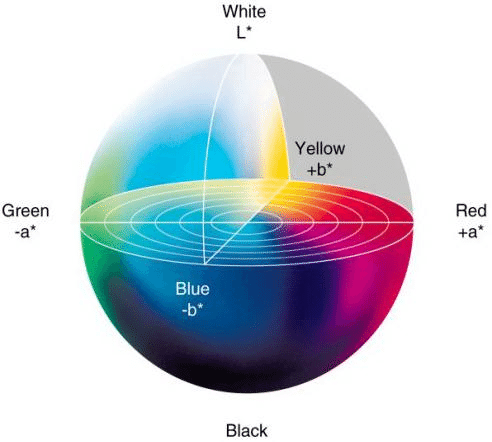
\includegraphics[width=3.5in]{CIELab}
    \caption[Przestrzeń barw CIELab - źródło:
    \url{https://www.flickr.com/photos/greenmambagreenmamba/4236391637}]
    {Przestrzeń barw CIELab.}
    \label{fig:CIELab}
  \end{figure}

  Zaletą zastosowania CIELab jest fakt, że jest ona najbardziej równomierną
  przestrzenią barw, co oznacza, że jeśli barwy znajdują się w jednakowej
  odległości od siebie w tej przestrzeni, to będą one postrzegane jako jednakowo
  różniące się od siebie. Powinno to zwiększyć skuteczność uczenia sieci oraz
  zapewnić bardziej realistyczne kolorowanie.

  Składowa \textit{L}, jako, że jest identyczna dla obrazu kolorowego jak i
  czarno-białego, stanowi w tym przypadku wejście sieci, na jej podstawie sieć
  odtwarza składowe \textit{A} oraz \textit{B}, które reprezentują przewidziane
  kolory dla obrazu wejściowego. W celu lepszego zrozumienia formatu przykładowa
  składowa \textit{L} została przedstawiona na Rysunku \ref{fig:przyklad_L}.
  Jak widać zawiera ona informacje wystarczające do rozróżnienia między sobą
  powierzchni oraz wydobycia ich kluczowych cech.

  \begin{figure}[ht]
    \centering
    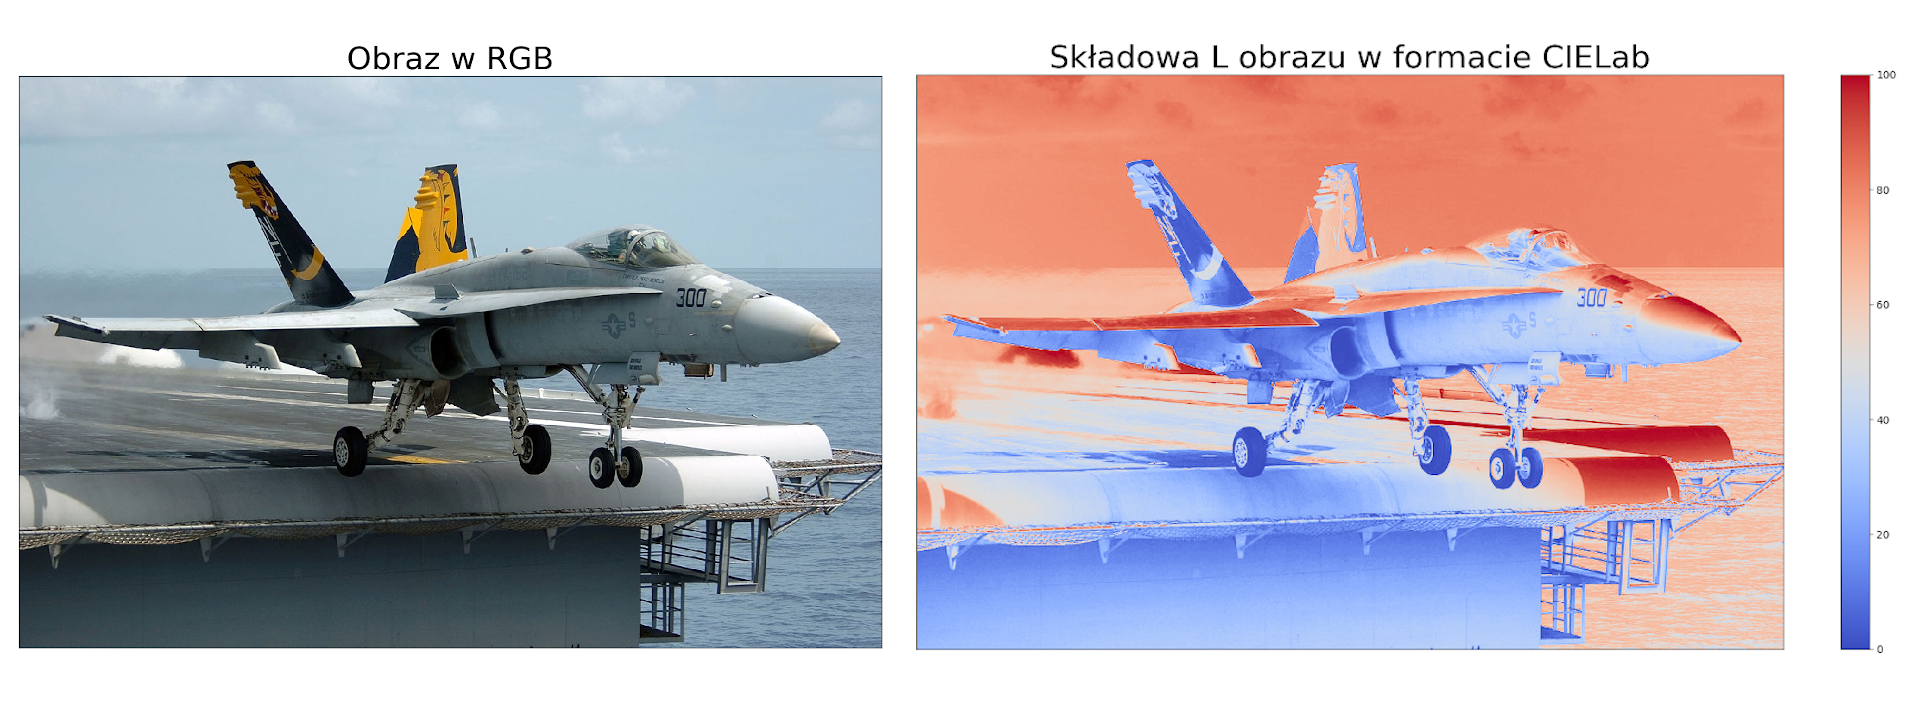
\includegraphics[width=6in]{rgb_i_L}
    \caption[Przykładowa składowa \textit{L} - źródło: Rysunek własny
    wykorzystujący:
    \url{https://fr.m.wikipedia.org/wiki/Fichier:An_F-A-18C_Hornet_launches_from_the_flight_deck_of_the_conventionally_powered_aircraft_carrier.jpg}]
    {Przykładowa składowa \textit{L}.}
    \label{fig:przyklad_L}
  \end{figure}

  Jako rozwiązanie podanej problematyki wpierw został oceniony autorski
  model, na jego podstawie zostało przeprowadzone porównanie skuteczności
  różnych konfiguracji, w których uczony był model. Do elementów poddanych
  testom należą algorytm optymalizacyjny, funkcja straty, funkcja aktywacja oraz
  sposób przetwarzania wstępnego danych treningowych.

\subsubsection{Model autorski} \label{model autorski}

  Opracowany przez nas model jest to FCN. Konwolucyjna część sieci składa się
  z 12 warstw splotowych
  mających na celu nauczyć się mapować składową wejściową \textit{L} na wyjściowe
  składowe \textit{A} i \textit{B}. Składowe wyjściowe muszą mieć takie same
  wymiary jak składowa wejściowe, co oznacza, że kluczowym było odpowiednie dobranie
  parametrów warstw takich jak \textit{padding} (pol. otoczka), \textit{stride}
  (pol. krok) oraz wielkość filtrów. Pełna architektura sieci została przedstawiona w
  Tabeli \ref{table:model_architecture}.
  \noindent\begin{table}[H]
    \center
    \begin{tabular}{|c | c | m{3.3em} | c | c | m{4em} | c | c| }
     \hline
     Nr & Warstwa & Rozmiar filtra & Stride & Padding & Batch Normalization &
     Fun. aktywacji & Ilość kanałów wej./wyj. \\ [0.5ex]
    \hline
    1 & Splotowa & 3x3 & 1 & 1 & Tak & ReLU & 1/32 \\ \hline
    2 & Splotowa & 3x3 & 1 & 1 & Tak & ReLU & 32/32 \\ \hline
    3 & Splotowa & 3x3 & 1 & 1 & Tak & ReLU & 32/32 \\ \hline
    4 & Splotowa & 3x3 & 1 & 1 & Tak & ReLU & 32/32 \\ \hline
    5 & Splotowa & 3x3 & 1 & 1 & Tak & ReLU & 32/64 \\ \hline
    6 & Splotowa & 3x3 & 1 & 1 & Tak & ReLU & 64/64 \\ \hline
    7 & Splotowa & 3x3 & 1 & 1 & Tak & ReLU & 64/64 \\ \hline
    8 & Splotowa & 3x3 & 1 & 1 & Tak & ReLU & 64/32 \\ \hline
    9 & Splotowa & 3x3 & 1 & 1 & Tak & ReLU & 32/32 \\ \hline
    10 & Splotowa & 1x1 & 1 & 0 & Tak & ReLU & 32/32 \\ \hline
    11 & Splotowa & 1x1 & 1 & 0 & Tak & ReLU & 32/32 \\ \hline
    12 & Splotowa & 1x1 & 1 & 0 & Nie & - & 32/2 \\ \hline
    \end{tabular}
    \caption{Architektura modelu podstawowego.}
    \label{table:model_architecture}
  \end{table}
  Pierwsza warstwa konwolucyjna rozkłada wejściowy kanał na 32 kanały, co
  pozwala wyciągnąć z niego jak najwięcej informacji o cechach obrazu. Warstwa
  ta ma wielkość filtra 3x3, tak więc aby zachować wymiar kanałów zostały
  zastosowane parametry $\textit{padding}=1$ oraz $\textit{stride}=1$.

  Kolejne trzy warstwy ekstraktują z wejściowych 32 kanałów najbardziej istotne
  cechy związane z powiązaniem treści obrazu z szacowanym kolorem jego powierzchni.
  Warstwy te na swoje wyjście przekazują po 32 kanały zawierające wykryte
  powiązanie pomiędzy pikselami kanałów wejściowych.

  Warstwa piąta rozciąga wejściowe 32 kanały na 64 kanały, dzięki temu kolejne
  2 warstwy przyjmujące na wejście te 64 kanały i przekazujące je na wyjście są
  w stanie wydobyć z obrazu cechy o większym poziomie abstrakcji, co znacznie
  zwiększa skuteczność działania sieci.

  Warstwa ósma ogranicza ilość kanałów w sieci z 64 do 32 wyciągając z nich
  cechy najbardziej przydatne do rozwiązania danej problematyki. Kanały te są
  następnie ponownie przetwarzane przez warwę z wielkością filtru 3x3, co ma
  służyć agregacji rozłożonych cech w bardziej spójną całość, która może być
  już składana w pożądane wyjście.

  Kolejne dwie warstwy w sieci są to warstwy konwolucyjne o wielkości filtru 1x1,
  odpowiadają one warstwom gęstym i mają na celu przekonwertowanie wartości
  funkcji aktywacji z poprzednich warstw na wartości kolorów odpowiadających
  pikseli w przestrzeni barw CIELab. Ostatnia warstwa, również z filtrem o
  wielkości 1x1 zwija 32 kanały otrzymywane na wejściu do 2 kanałów odpowiadających
  składowym \textit{A} oraz \textit{B}, które stanowią pożądany rezultat działania
  sieci.

  Po wszystkich, oprócz ostatniej, warstwach konwolucyjnych znajdują się dodatkowo
  warstwa BatchNorm oraz warstwa funkcji aktywacji ReLU mające na celu
  ustabilizować proces uczenia oraz zwiększyć jego efektywność.

\subsubsection{BatchNorm} \label{BatchNorm}

  Warstwa Batch Normalization została przedstawiona w 2015 roku przez S. Ioeffe
  oraz C. Szegedy jako odpowiedź
  na problem zmieniającej się podczas uczenia dystrybucji wartości wejść
  każdej z warstw sieci \cite{BatchNorm}. Ma ona na celu usprawnić i ustabilizować
  trening sieci poprzez normalizację wartości podawanych na funkcje aktywacji.
  Zmienna dystrybucja tych wartości znacznie spowalnia i utrudnia proces uczenia
  poprzez potrzebę przemyślanego inicjowania
  wag sieci w celu zwiększenia prawdopodobieństwa nakierowania modelu na pożądane
  rozwiązania w trakcie procesu uczenia oraz przez
  konieczność używania mniejszych wartości współczynnika uczenia, aby
  przeciwdziałać problemom zanikającego oraz wybuchającego gradientu
  \cite{exploding_vanishing_grad}.

  Problemy te zostały już zauważone i opisane w 1994 roku przez Y. Bengio
  oraz jego współpracowników \cite{exploding_vanishing_grad}. Dowodzą oni, że:
  \begin{quote}
    % 'Gradient descent becomes increasingly inefficient when the
    % temporal span of the dependencies increases'
    'Metoda gradientu prostego staje się coraz bardziej nieefektywna, gdy
    rośnie czasowy zakres zależności'
  \end{quote}
  Wskazują także, że problemy powstają podczas treningu DNN w fazie wstecznej
  propagacji błędu, kiedy to gradient pochodzący z głębszych warstw przechodzi
  wielokrotnie przez operacje mnożenia macierzowego. Jeśli wartość gradientu
  jest niewielka, to z każdą operacją mnożenia staje się jeszcze mniejsza, aż
  maleje do takich wartości, które nie umożliwiają modelowi uczenia się, a jeśli
  wartość ta jest wysoka to, wraz z przechodzeniem przez kolejne warstwy, rośnie
  jeszcze bardziej co przy bardzo dużych wartościach może doprowadzić do
  destabilizacji procesu uczenia. Są to zjawiska zdecydowanie niepożądane i z
  tego powodu powstało wiele rozwiązań, aby im przeciwdziałać takich jak
  ograniczanie maksymalnej wartości gradientu (ang. gradient clipping) albo
  zastosowanie warstw BatchNorm.

  Zastosowanie warstw BatchNorm sprawia, że podczas uczenia metodą mini-batch
  (pol. małych paczek) każda paczka jest
  normalizowana w sposób zapewniający zerową wartość średnią oraz
  równą jedności wariancję na przestrzeni wszystkich kanałów wejściowych.
  Zaletą takiego podejścia jest poprawienie przepływu korygującego gradientu
  przez kolejne warstwy sieci podczas fazy wstecznej propagacji błędu. Ponadto
  warstwy BatchNorm zapewniają większą odporność sieci na niekorzystnie zainicjowane
  wagi początkowe modelu.

  Użycie tych warstw w modelu podstawowym tuż za warstwami ReLU pozwoliło
  uzyskać bardziej korzystną zbieżność modelu oraz lepsze rezultaty końcowe.
  Ocenione zostało też rozwiązania, w którym warstwy BatchNorm znajdują się
  przed warstwami funkcji aktywacji, lecz dało ono gorsze rezultaty, niż
  podejście wspomniane jako pierwsze.

\subsubsection{Dropout} \label{Dropout}

  W trakcie pracy nad ostatecznym modelem podstawowym sprawdzona została
  skuteczność zastosowania warstw Dropout \cite{dropout}. Warstwy te w trakcie
  treningu dezaktywują część neuron aby przeciwdziałać efektowi przeuczania
  się sieci oraz zapewniać wydajny sposób łączenia wielu różnych architektur
  sieci stworzonych do jednego celu w jednolitą całość o skuteczności większej
  niż poszczególne sieci osobno.

  Wybór neuronów, dla których w danej iteracji treningu nie zostaną
  zaktualizowane wagi odbywa się z pewnym prawdopodobieństwem określonym
  podczas inicjalizacji modelu. Dezaktywowanie neuronów można interpretować jak
  przerywanie tymczasowo wszystkich połączeń danego neuronu, zarówno wejściowych
  jak i wyjściowych. Takie działania są równoznaczne z wyselekcjonowaniem z modelu
  mniejszej sieci i trenowaniu wyłącznie jej w aktualnej iteracji. Wagi tej
  podsieci są wtedy współdzielone z modelem źródłowym.
  Jako rezultat uzyskuje się model o znacznie ulepszonych zdolnościach generalizacji.

  Zastosowanie tych warstw w modelu nie przyniosło wyraźnego polepszenia rezultatów
  sieci. W przypadku danej problematyki oraz obranego podejścia do jej rozwiązania,
  przeuczenie sieci nie stanowi wyraźnego zagrożenia, a zastosowanie Dropout
  wiąże się z utratą części informacji kluczowych do odpowiedniego
  generowanie kolorów dla wejściowych obrazów. Model powinien nauczyć się jak
  największej różnorodności kolorów, a Dropout przeciwdziała uczeniu się
  nadmiernej ilości cech przez sieć, co wpływa niekorzystnie na otrzymywane
  rezultaty końcowe. Podczas testów skuteczności tych warstw zostały one umieszczone
  za warstwami BatchNorm. Wizualizacja skutków tej decyzji dla różnych wartości
  parametru \textit{p} (prawdopodobieństwo dezaktywowania dla każdego neuronu sieci)
  wraz z rozważeniem
  pozostałych czynników wpływających na efektywność sieci znajdują się w
  punkcie \ref{Rezultaty} związanym z rezultatami modelu podstawowego.

\subsubsection{Modyfikacja rozdzielczości}

  W modelach FCN powszechnie stosuje się różne metody zmiany rozdzielczości
  kanałów przechodzących przez sieć, najczęściej są do operacje poolingu mające
  na celu zredukować przestrzenną wielkość reprezentacji cech wyciągniętych z
  obrazu poprzez wyciągnięcie najbardziej istotnych wartości funkcji aktywacji z
  określonych obszarów reprezentacji w celu zredukowania rozmiaru
  sieci, a co za tym idzie, zmniejszenia ilości obliczeń koniecznych do wykonania
  przez sieć.

  Ponadto pooling wspomaga adaptację modelu do zmiennego położenia
  kluczowych wzorów rozpoznawanych przez sieć na obrazie wejściowym. Cecha ta
  zwana jest niezmiennością od translacji (ang. transaltion invariance). Jest
  ona rezultatem dokonywania operacji, takich jak wyliczanie wartości maksymalnej
  z poszczególnych obszarów, dzięki którym zmienne położenie wartości
  selekcjonowanej, a co tym idzie, zmienne położenie ekstraktowanej cechy w obrębie
  danego obszaru nie wpływa na końcową postać reprezentacji przestrzennej obrazu
  wejściowego po przejściu przez warstwę poolingu. Przykładowe operacja poolingu
  została przedstawiona na Rysunku \ref{fig:pooling}.

  \begin{figure}[h]
   \centering
   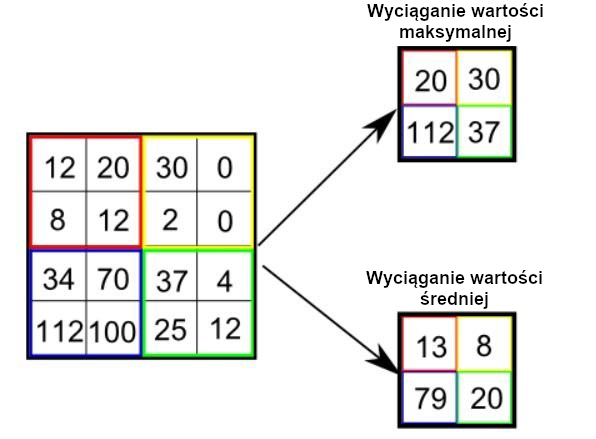
\includegraphics[width=5in]{pooling}
   \caption[Przykładowe operacje warstwy poolingu - źródło: Rysunek własny]{Przykładowe operacje warstwy poolingu}
   \label{fig:pooling}
  \end{figure}

  W modelu autorskim warstwy poolingu nie zostały zastosowane, aby uniknąć utraty
  kluczowych informacji przestrzennych koniecznych to właściwego wygenerowanie
  możliwych barw obrazu.

\subsubsection{Wykorzystywany zbiór treningowy}

  Do uczenia modelu został wykorzystany zbiór danych CIFAR-10 stworzony przez
  A. Krizhevsky oraz zaprezentowany w 2009 roku \cite{cifar-10}.
  Składa się on z 60000 obrazów w przestrzeni kolorów RGB o rozdzielczości 32 x 32 piksele.
  Spośród tych obrazów 10000 z nich zostało wykorzystanych jako zbiór
  walidacyjny do śledzenia skuteczności treningu modelu. Przykładowe obrazy
  ze zbioru danych zostały przedstawione na Rysunku \ref{fig:cifar10}.

  \begin{figure}[h]
   \centering
   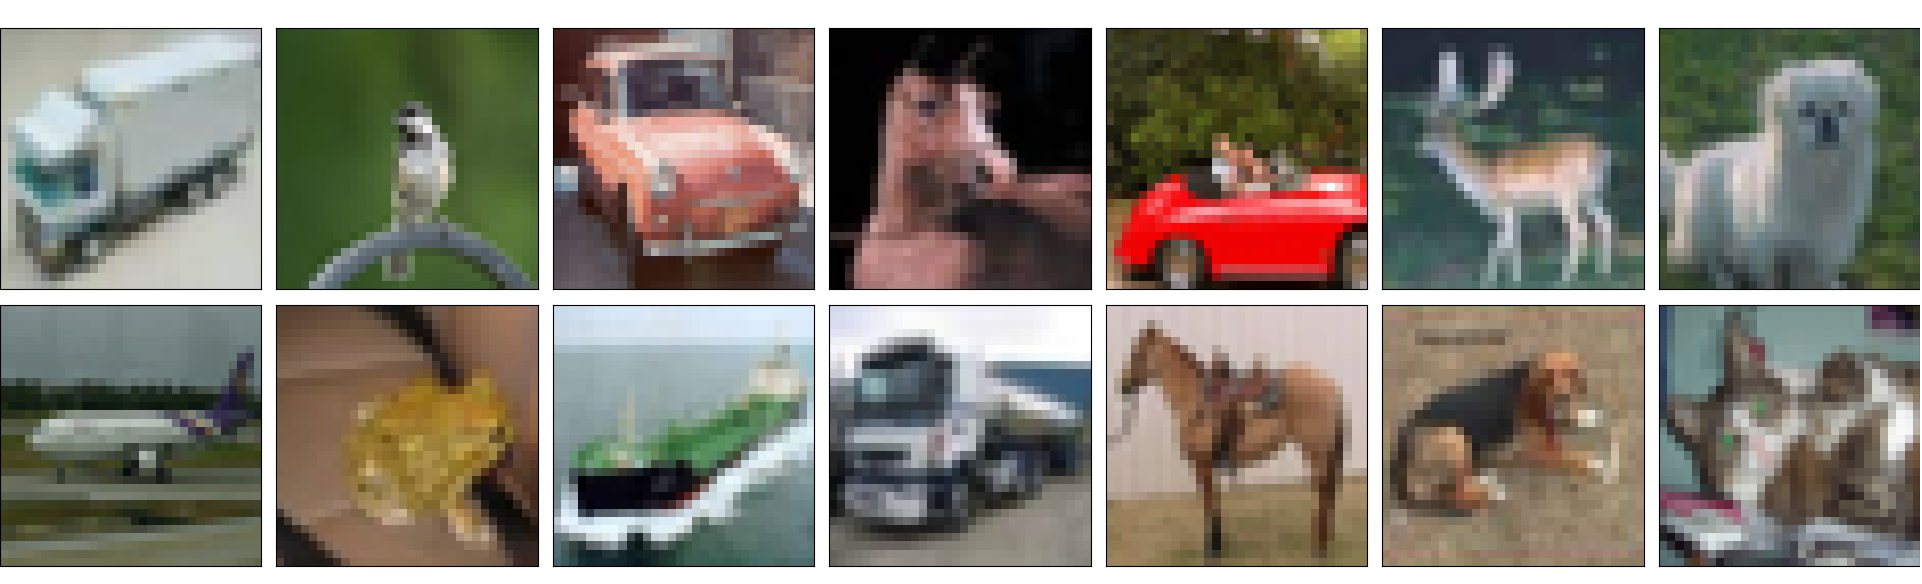
\includegraphics[width=5.5in]{cifar10}
   \caption[Przykładowe obrazy z CIFAR-10 - źródło: Rysunek własny]
   {Przykładowe obrazy z CIFAR-10}
   \label{fig:cifar10}
  \end{figure}

  Zaletą CIFAR-10 jest niewielka rozdzielczość obrazów co pozwala na mniej
  złożony model oraz szybszy proces uczenia, który można skutecznie przeprowadzić
  nawet przy ograniczonych możliwościach obliczeniowych. Ponadto zbiór ten składa
  się z obrazów dzielących się na 10 klas, tak mała różnorodność klas, a co za
  tym idzie, stosunkowo niewielka ilość możliwych obiektów pojawiających się
  na zdjęciach powinna ułatwić sieci wyuczenie się właściwych barw dla
  identyfikowanych powierzchni. Z drugiej strony mała ilość klas może niekorzystnie
  wpłynąć na umiejętność generalizacji modelu, jednakże obrazy z CIFAR-10
  przedstawiają zróżnicowane otoczenia zawierające obiekty nie kwalifikujące
  się do żadnej klasy, co powinno umożliwić wyuczenia się generalizacji przez
  sieć.

\subsubsection{Przetwarzanie wstępne danych} \label{Przetwarzanie wstępne danych}

  Przed podaniem na wejście sieci obrazy uczące były wpierw poddawane
  przetwarzaniu wstępnemu mającemu na celu doprowadzić do szybszego oraz
  stabilniejszego treningu modelu. Przetwarzanie wstępne jest kluczowe, gdyż
  wartości o jakie aktualizowane są wagi neuronu zależą w dużej mierze od
  wartości wejść tego neuronu. W przypadku gdy przedziały wartości tych wejść
  nie są jednolite, to może wystąpić duża różnica w tempie aktualizacji wag
  sieci, niektóre wagi będą zmieniane o wiele szybciej niż inne co może spowodować
  destabilizację treningu. Przeskalowanie wszystkich wartości wejściowych do jednakowych
  przedziałów, o niewielkiej wartości maksymalnej i minimalnej oraz wartości
  średniej zbliżonej do zera zmniejsza możliwość wystąpienia tego problemu
  oraz sprzyja ujednoliceniu tempa uczenia się przez sieć rozpoznawania różnych cech.
  Ponadto brak przeskalowania wejść może doprowadzić do zjawisk wybuchającego
  oraz zanikającego gradientu.

  % Przeskalowanie wszystkich wartości wejściowych do jednakowych
  % przedziałów, o niewielkiej wartości maksymalnej i minimalnej oraz wartości
  % średniej zbliżonej do zera, sprzyja ujednoliceniu tempa uczenia się przez sieć
  % rozpoznawania różnych cech.
  \noindent
  W ramach badania rozwiązania przetestowane zostały różne metody przetwarzania
  wstępnego zarówno danych wejściowych jak i pożądanej odpowiedzi:
  \begin{itemize}
  \item Normalizacja danych na przestrzeni całego zbioru danych z użyciem wartości
  maksymalnej oraz minimalnej całego zbioru, tak aby wartości pikseli danej składowej
  dla każdego obrazu zawierały się w przedziale od -0.5 do 0.5.
  \item Standaryzacja danych na przestrzeni całego zbioru danych z użyciem wartości
  średniej oraz odchylenia standardowego całego zbioru, tak aby uzyskać wartość
  średnią równą w przybliżeniu zero oraz jednostkowe odchylenie standardowe.
  \item Zastosowanie rozmycia gaussowskiego(ang. Gaussian blur) o różnej
  wielkości filtru Gaussowskiego.
  % \item Przepuszczenie składowej przez filtr Gaussa o różnej wielkości filtru.
  \end{itemize}

  Rozmycie gaussowskie, zwane także wygładzaniem gaussowskim (ang. Gaussian smoothing),
  jest to operacja polegająca na modyfikacji obrazu z użyciem filtru Gaussa.
  Stosuje się je w celu rozmycia detali na przetwarzanym obrazie, a także by
  ograniczyć ilość występujących na nim zakłóceń oraz szumów. Jest ono powszechnie
  stosowane w fazie przetwarzania wstępnego danych graficznych. W praktyce
  operacja ta sprowadza się do dokonywania splotu kolejnych fragmentów obrazu
  z funkcją Gaussa. Zastosowanie jej na danych wejściowych miało na celu
  zmniejszenie znaczenie detali na obrazie oraz ułatwienie sieci nauczenia się
  rozróżniania rozmaitych powierzchni oraz wzorców.

  Wymienione metody przetwarzania były stosowane w różnych połączeniach oraz
  konfiguracjach zarówno na składowej \textit{L}, jak i składowych \textit{A}
  oraz \textit{B}, a uzyskane wyniki opisane zostały w punkcie \ref{Rezultaty}

\subsubsection{Przetwarzanie końcowe danych}  \label{Przetwarzanie końcowe danych}

  Jeśli w trakcie procesu uczenia były stosowane zabiegi przetwarzania
  wstępnego danych wejściowych to podczas testowania modelu dane testowe również
  muszą być przetworzone w ten sam sposób, aby zapewnić poprawną pracę sieci.
  To samo dotyczy się danych wyjściowych sieci, jeśli podczas treningu z nadzorem
  pożądane wyjście było w pewien sposób przetworzone wstępnie to sieć uczy się
  odtwarzać te wyjście tak samo przetworzone, aby uzyskać oczekiwany efekt
  końcowy należy dokonać operacji odwrotnych do tych zastosowanych w fazie
  przetwarzania wstępnego. Przykładowo jeśli pożądana odpowiedź w procesie
  uczenia była normalizowana to podczas testów sieci jej wyście należy
  zdenormalizować, aby uzyskać oczekiwany rezultat. Jednakże my dla rozważanej
  problematyki proponujemy metodę alternatywną.

  Polega ona na uwydatnianiu kolorów wygenerowanych przez sieć dla wysokich
  wartości naświetlenia - składowej \textit{L}. Może być ona stosowana
  niezależnie od metody przetwarzania wstępnego danych wejściowych. Algorytm
  polega na przeskalowaniu pikseli składowych \textit{A} i \textit{B} tak, aby
  ich wartości mogły pokryć cały dostępny przedział wartości, ale dla danego
  piksela jego przedział jest ograniczony proporcjonalnie do stosunku wartości
  tego piksela w składowej \textit{L} do maksymalnej możliwej wartości pikseli
  składowej \textit{L}.

  Dla przykładu załóżmy, że wartość danego pikselu dla składowej \textit{A}
  wynosi 70, dla składowej \textit{B} wynosi -20, a dla składowej \textit{L} 80.
  Przedział wartości składowych \textit{A} i \textit{B} jest od -127 do 128, a
  składowej \textit{L} od 0 do 100. W następnym kroku znajdowana jest maksymalna
  absolutna wartość składowych \textit{A} i \textit{B} dla aktualnego obrazu.
  Załóżmy, że dla \textit{A} wynosi ona 90, a dla \textit{B} 60.
  Następnie piksele składowych \textit{A} i \textit{B} są dzielone przez
  swoje maksymalne wartości, a następnie rozciągnięte na cały dostępny przedział
  przez pomnożenie przez odpowiedni czynnik, czynnik ten jest z przedziału
  od 0 do 127 i jest wprost proporcjonalny do stosunku aktualnego piksela
  składowej \textit{L} do maksymalnej wartości \textit{L}, oznacza to, że jeśli
  dany piksel \textit{L} jest równy 100 to czynnik jest równy 127, a jeśli
  dany piksel \textit{L} jest równy 50 to wartość czynnika znajduje się w
  połowie swojego przedziału i równy jest 63,5.

  \noindent
  Dla podanych założeń otrzymujemy następujące nowe wartości piksela składowej \textit{A}
  ($p_{n}^{A}$) i piksela składowej \textit{B} ($p_{n}^{B}$):
  \begin{equation}
  p_{n}^{A} = \frac{70}{90} * 127 * \frac{80}{100} = 79.02
  \end{equation}
  \begin{equation}
  p_{n}^{B} = \frac{-20}{60} * 127 * \frac{80}{100} = -33.87
  \end{equation}

  \noindent
  Algorytm konwertowanie pikseli danej składowej można przedstawić wzorem:
  \begin{equation}
  S_{i, j}^{n} = \frac{S_{i, j}^{p}}{max\{abs\{S\}\}} * 127 * \frac{L_{i, j}}{100}
  \end{equation}

  \noindent
  Gdzie:
  \begin{itemize}
    \item $S$ - Konwertowana składowa będąca dwuwymiarowa macierzą pikseli.
    \item $S_{i, j}^{n}$ - Nowa wartość piksela (i, j) dla danej składowej.
    \item $S_{i, j}^{p}$ - Stara wartość piksela (i, j) dla danej składowej.
    \item $L_{i, j}$ - Wartość piksela (i, j) składowej jasności.
  \end{itemize}

  Zastosowanie powyższego algorytmu pozwoliło uzyskać bardziej zadawalające
  rezultaty działania modelu poprzez faworyzowanie kolorów tworzonych przez sieć
  dla powierzchni o dużej wartości jasności, jako, że wysoka jasność oferuje
  bardziej intensywne barwy. Kolorystyka powierzchni ciemnych pozostaje
  przytłumiona, jako, że brak naświetlenia ogranicza natężenie kolorów.

\subsubsection{Augmentacja danych}

  W celu skutecznego treningu modelu potrzebny jest odpowiednio duży i różnorodny
  zbiór treningowy. W obliczu problemu niewystarczającej ilości danych stosuje
  się metody zwane augmentacją danych pozwalające poszerzyć zbiór obrazów uczących
  poprzez dodawanie nowych informacji do obrazów będących podstawą zbioru tworząc
  w ten sposób nowe obrazy, które mogą być wykorzystane w treningu. Augmentacja
  danych przeciwdziała uczeniu się przez sieć nieistotnych wzorów i cech takich jak
  orientacja obiektu, jego umiejscowienie albo rozmiar. Dzięki temu model jest
  w stanie dogłębniej analizować obrazy wejściowe ucząc się rozpoznawać cechy
  o coraz to większym poziomie abstrakcji co przekłada się na o wiele lepiej
  rozwiniętą zdolność modelu do generalizacji danej problematyki.

  \noindent
  Do augmentacji stosuje się proste przekształcenia obrazu takie jak:
  \begin{itemize}
  \item Rotacja obrazu o wybrany kąt.
  \item Odbicie obrazu względem osi pionowej.
  \item Obcinanie skrajnych fragmentów obrazów (ang. crop).
  \item Zmiana odcienia oraz saturacji barw obrazu.
  \item Przybliżanie albo oddalanie treści obrazu.
  \item Modyfikacja rozdzielczości obrazu poprzez jego rozciąganie lub ściskanie.
  \item Tworzenie niewielkich ubytków w obrazach w losowych miejscach (ang. coarse dropout).
  \end{itemize}

  Należy jednak pamiętać, że nie wszystkie metody augmentacji nadają się do każdego zbioru
  danych, kluczowe jest, aby wybrać takie operacje, które poszerzają zbiór
  uczący o dane niosące znaczące oraz sensowne informacje patrząc z punktu wybranej
  problematyki oraz nie przesłaniają wzorców kluczowych do wyuczenia przez sieć.
  W przypadku zagadnienia kolorowania czarno-białych obrazów kluczową informacją
  jest kolor analizowanej powierzchni oraz jej cechy charakterystyczne, z tego
  powodu, do treningu modelu podstawowego nie zostały wykorzystane żadne metody
  augmentacji wpływające na barwy albo jasność obrazów. Wykluczone zostały również takie
  metody jak tworzeniu ubytków w obrazach, gdyż powoduje to niepotrzebną utratę
  informacji.
  W związku z tym, że wykorzystany zbiór CIFAR-10 posiada dużą ilość obrazów
  to w procesie uczenia została wykorzystana jedynie augmentacja poprzez
  odbicie obrazu względem osi pionowej z prawdopodobieństwem równym 50\%.

  % W zagadnieniu kolorowania czarno-białych obrazów informacjami najważniejszymi
  % są wartości pikseli powiązane z daną powierzchnią oraz cechy charakterystyczne
  % tych powierzchni, z tego powodu, aby ograniczyć straty
  % w procesie uczenia nie zastosowano żadnej
  % metody związanej ze zmianą barw obrazu wejściowego, jednocześnie nie można
  % było sobie pozwolić

\subsubsection{Funkcje kosztów} \label{Funkcje kosztów}
  % Bez teorii
  Kluczem do właściwego funkcjonowania modelu jest wybór odpowiedniej funkcji
  kosztu. W przypadku problematyki kolorowania czarno-białych obrazów ważne
  jest, aby wybrana funkcja kosztu uwzględniała specyficzną naturę problemu,
  gdzie dla niektórych przypadków właściwych jest wiele odpowiedzi. Jako
  przykład można podać taki obiekt jak samochód, który może być zarówno
  zielony, czerwony jak i żółty, każdy z tych kolorów powinien być oceniony
  jako właściwy, a wartość błędu wyliczona z użyciem funkcji kosztu dla tak
  wybranych przez sieć kolorów powinna odpowiednio to wskazywać. W ramach
  poszukiwań najbardziej odpowiedniej funkcji kosztu przetestowane zostały
  następujące funkcje.

  \begin{enumerate}[leftmargin=*]
  \item MSELoss (ang. Mean Squared Error Loss) - koszt oparty na błędzie średniokwadratowym
  przedstawiony funkcją:
  \begin{equation}
  Koszt = \frac{1}{n}\sum_{i=0}^{n} (x_{i} - y_{i})^2
  \end{equation}

  % \noindent
  % gdzie $x$ są to składowe \textit{A} oraz \textit{B} przewidziane przez sieć,
  % a $y$ to rzeczywiste \textit{A} i \textit{B}.

  \noindent
  Po dopasowaniu równania MSELoss do rozważanej problematyki otrzyma się:
  \begin{equation}
  Koszt = \frac{1}{n}\frac{1}{m}\sum_{i=0}^{n}\sum_{j=0}^{m} ((A_{i, j}^{P} - A_{i, j}^{R})^2 + (B_{i, j}^{P} - B_{i, j}^{R}))^2
  \end{equation}

  % \noindent
  % gdzie $(A_{i, j}^{R}$ i $(B_{i, j}^{R}$ są to rzeczywiste wartości składowych
  % \textit{A} i \textit{B} dla pikselu obrazy o współrzędnych $(i, j)$, a
  % $(A_{i, j}^{P}$ i $(B_{i, j}^{P}$ są to wartości przewidziane przez sieć.

  \item L1Loss zwany także MAELoss (ang. Mean Absolute Error Loss) - koszt oparty na
  średnim błędzie bezwzględnym dany funkcją:
  \begin{equation}
  Koszt = \frac{1}{n}\sum_{i=0}^{n} |x_{i} - y_{i}|
  \end{equation}
  % gdzie $x$ są to składowe \textit{A} oraz \textit{B} przewidziane przez sieć,
  % a $y$ to rzeczywiste \textit{A} i \textit{B}.

  \noindent
  Równanie L1Loss dla rozważanego zagadnienia:
  \begin{equation}
  Koszt = \frac{1}{n}\frac{1}{m}\sum_{i=0}^{n}\sum_{j=0}^{m} (|A_{i, j}^{P} - A_{i, j}^{R}| + |B_{i, j}^{P} - B_{i, j}^{R}|)
  \end{equation}
  % gdzie $x$ są to składowe \textit{A} oraz \textit{B} przewidziane przez sieć,
  % a $y$ to rzeczywiste \textit{A} i \textit{B}.

  \item SmoothL1Loss - zwany także \textit{Huber loss}, odmiana L1Loss przedstawiona w
  2015 roku przez R. Girshick \cite{SmoothL1Loss}. Jej zaletami są mniejsza
  czułość na elementy odstające (ang. outliner) i zmniejszona szansa na wystąpienie
  zjawiska eksplodującego gradientu.
  SmoothL1Loss przedstawiony jest funkcją:
  \begin{equation}
  Koszt = \frac{1}{n}\sum_{i=0}^{n} z_{i}
  \end{equation}

  \noindent
  gdzie $z_{i}$ dane jest:
  \begin{equation}
  z_{i} = \begin{cases}
               0.5(x_{i} - y_{i})^2 \text{, jeśli } |x_{i} - y_{i}| < 1 \\
               |x_{i} - y_{i}| - 0.5 \text{, w pozostałych przypadkach}
            \end{cases}
  \end{equation}

  \noindent
  Zastosowanie SmoothL1Loss do modelu podstawowego da następującą funkcję:
  \begin{equation}
  Koszt = \frac{1}{n}\sum_{i=0}^{n} (z_{i} + k_{i})
  \end{equation}

  \noindent
  gdzie $z_{i}$ dane jest:
  \begin{equation}
  z_{i} = \begin{cases}
               0.5(A_{i, j}^{P} - A_{i, j}^{R})^2 \text{, jeśli } |A_{i, j}^{P} - A_{i, j}^{R}| < 1 \\
               |A_{i, j}^{P} - A_{i, j}^{R}| - 0.5 \text{, w pozostałych przypadkach}
            \end{cases}
  \end{equation}

  \noindent
  a $k_{i}$ dane jest:
  \begin{equation}
  z_{i} = \begin{cases}
               0.5(B_{i, j}^{P} - B_{i, j}^{R})^2 \text{, jeśli } |B_{i, j}^{P} - B_{i, j}^{R}| < 1 \\
               |B_{i, j}^{P} - B_{i, j}^{R}| - 0.5 \text{, w pozostałych przypadkach}
            \end{cases}
  \end{equation}

  \end{enumerate}
  \noindent
  Gdzie:
  \begin{itemize}
    \item $x$ są to składowe \textit{A} oraz \textit{B} przewidziane przez sieć.
    \item $y$ to rzeczywiste składowe \textit{A} i \textit{B}.
    \item $A_{i, j}^{R}$ i $B_{i, j}^{R}$ są to rzeczywiste wartości składowych
    \textit{A} i \textit{B} dla pikselu obrazy o współrzędnych $(i, j)$.
    \item $A_{i, j}^{P}$ i $B_{i, j}^{P}$ są to wartości składowych
    \textit{A} i \textit{B} przewidziane przez sieć dla pikselu obrazy o
    współrzędnych $(i, j)$.
  \end{itemize}

  \noindent
  Szczegółowy opis skutków zastosowanie poszczególnych funkcji kosztów umieszczony
  został w punkcie \ref{Rezultaty}.

\subsubsection{Funkcje aktywacji}
  % ReLU
  W wyborze odpowiednej funkcji aktywacji kierowaliśmy się badaniami przeprowadzonymi
  przez B. Xu oraz jego współpracowników \cite{evaluatiuon_of_relu}. Testowali
  oni skuteczność takich funkcji jak ReLU, Leaky ReLU (pol. przepuszczające ReLU),
  PReLU (ang. Parametric ReLU) oraz RReLU (ang. Randomized Leaky ReLU) w
  zagadnieniu klasyfikacji treści obrazów. Bazując na otrzymanych przez nich
  rezultatach zdecydowaliśmy się wykorzystać w rozważanej problematyce funkcję
  aktywacji ReLU, przedstawioną na Rysunku \ref{fig:relu}

  \begin{figure}[h]
   \centering
   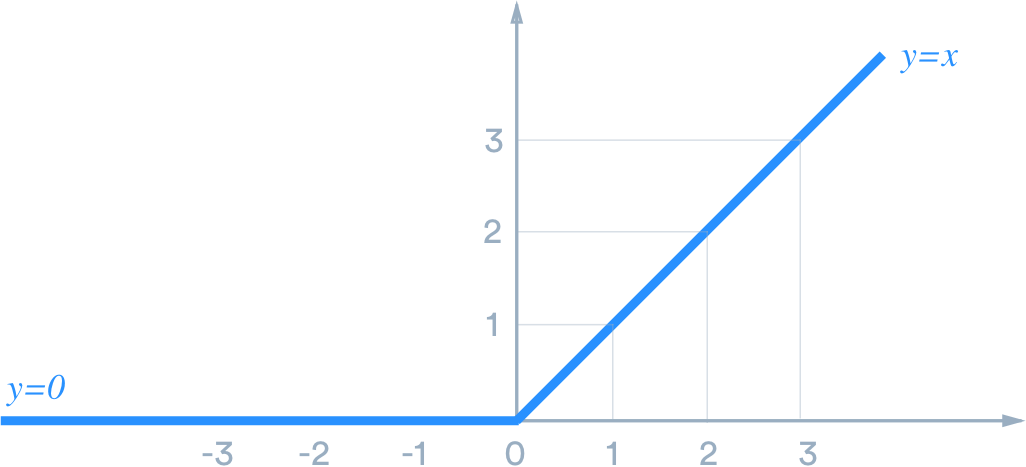
\includegraphics[width=4in]{relu}
   \caption[Funkcja aktywacji ReLU - źródło: \url{https://pytorch.org/docs/stable/_images/ReLU.png}]
   {Funkcja aktywacji ReLU}
   \label{fig:relu}
  \end{figure}

  Funkcja ta posiada wiele zalet takich jak przyspieszenie procesu zbieganie się stanu
  sieci do stanu pożądanego poprzez brak ograniczeń na maksymalną wartość
  funkcji oraz niska złożoność obliczeniowa.
  Ponadto funkcja ta, w związku z zerową wartością dla ujemnych argumentów,
  zapewnia aktywację neuronów modelu tylko wtedy, gdy analizują one wzorce
  kluczowe dla nich samych oraz danego zagadnienia, zwiększa to odporność modelu na
  szumy wejściowe oraz przeuczanie, a także poprawia zdolności predykcyjne sieci.

  Jednakże stosowanie ReLU tworzy zagrożenie blokowanie się procesu uczenia,
  jeśli dojdzie do sytuacji, w której wagi modelu dojdą do stanu, gdzie wartość
  aktywacji będzie zbliżona do zera. Spowoduje to zerową wartość gradientu
  podczas fazy wstecznej propagacji błędu powodując wstrzymanie się procesu
  aktualizowania wag modelu, a w rezultacie, nieefektywny proces uczenia.
  Pomimo to jednak zostaliśmy przy wyborze funkcji ReLU wierząc, że pozostałe
  zabiegi takie jak zastosowanie warstw BatchNorm pozwolą zminimalizować
  niepożądane efekty tego zjawiska.

\subsubsection{Algorytmy optymalizacyjne} \label{Algorytmy optymalizacyjne}
  % Bez teorii
  % TODO: Może dać bardziej szczegółowy opis
  % TODO: Zacytować twórców Adam i Adagrad, linki do paperów są w dokumentacji
  % pytorcha o tych algorytmach
  Podczas planowanie treningu modelu należy zdecydować się na odpowiedni
  algorytm optymalizacyjny, właściwa decyzja pozwala uniknąć zatrzymania się
  procesu uczenia w lokalnych minimach co zwiększa końcową dokładność oraz
  skuteczność modelu.
  Podczas badań przetestowane zostały różne algorytmy optymalizacyjne,
  a uzyskane rezultaty zostały szczegółowo opisane oraz porównane w punkcie
  \ref{Rezultaty}.\newline
  Wykorzystane zostały następujące algorytmy:
  \begin{itemize}
    \item Adam (ang. Adaptive Moment Estimation)
    \item Adagrad (ang. Adaptive Gradient Algorithm)
    \item SGD (ang. Stochastic Gradient Descent)
  \end{itemize}

  \noindent
  Przeprowadzone zostały także poszukiwania najbardziej odpowiednich hiperparametrów
  dla wymienionych algorytmów w celu osiągnięcia jak największej ich skuteczności
  w rozwiązaniu rozważanej problematyki.

% TODO: Od tego momentu było ekspres pisanie, wiec może do zredagowania
\subsubsection{Trening}

Model trenowaliśmy paczkami o wielkości 128 obrazów, cała epoka składała się z
50000 obrazów. Przed każdą epoką zbiór treningowy był przetasowywany, aby
przeciwdziałać przeuczaniu się sieci. Aby znaleźć najbardziej zadowalające rozwiązanie
przetestowane zostały różne konfiguracje treningowe, możliwe zmienne elementy
konfiguracji to algorytmy optymalizacyjne opisane w punkcie
\ref{Algorytmy optymalizacyjne}, funkcje kosztów opisane w punkcie \ref{Funkcje kosztów},
rodzaje przetwarzania wstępnego opisane w punkcie \ref{Przetwarzanie wstępne danych} oraz
skutki zastosowanie takich warstw jak Dropout (punkt \ref{Dropout}) oraz BatchNorm
(punkt \ref{BatchNorm}). Jako funkcja aktywacji wybrana została funkcja ReLU.
Dla różnych konfiguracji została także przedstawiona charakterystyka porównawcza.


\subsubsection{Rezultaty} \label{Rezultaty}

 Uzyskane wyniki są w znacznej mierze zależne od wybranej konfiguracji.
 Najbardziej satysfakcjonujące rezultaty uzyskane przez model zostały
 przedstawione na Rysunku \ref{fig:best_result}

 \begin{figure}[ht]
   \centering
   \subfloat[Obraz spoza zbioru uczącego]{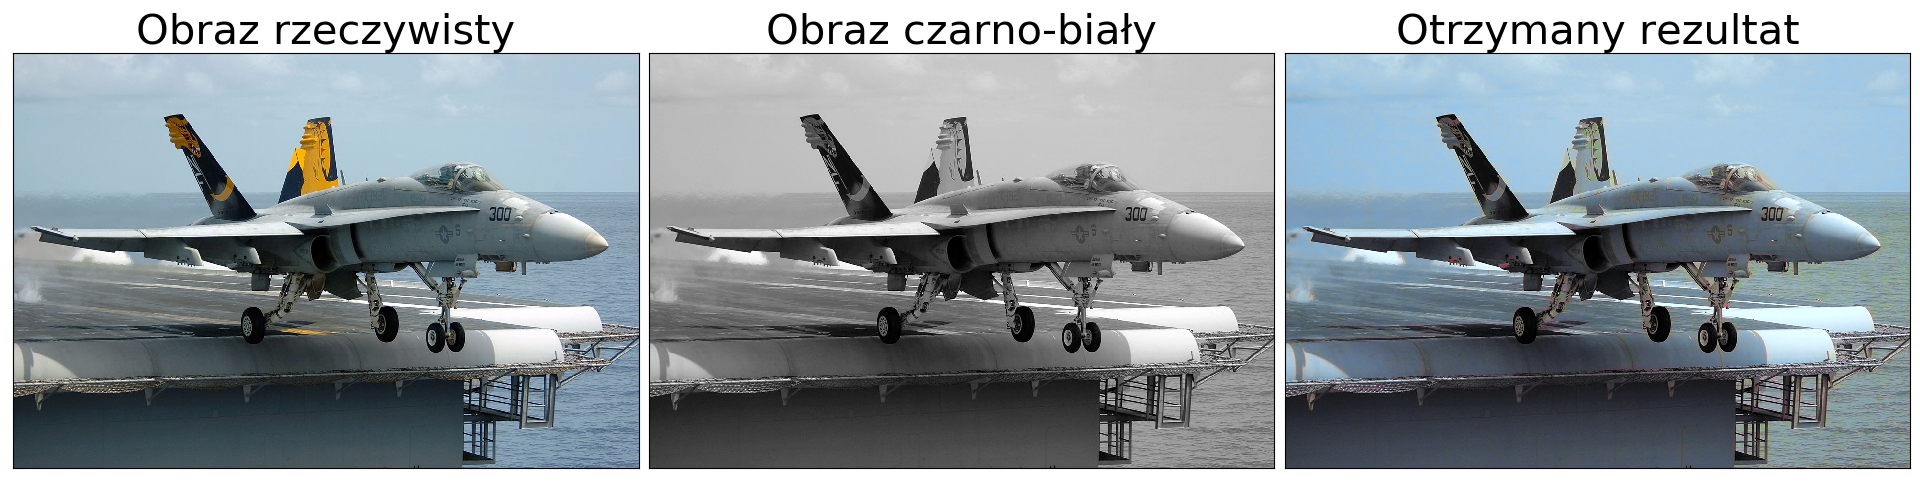
\includegraphics[width = 4.5in]{best_results_plane}} \\
   \subfloat[Obraz spoza zbioru uczącego]{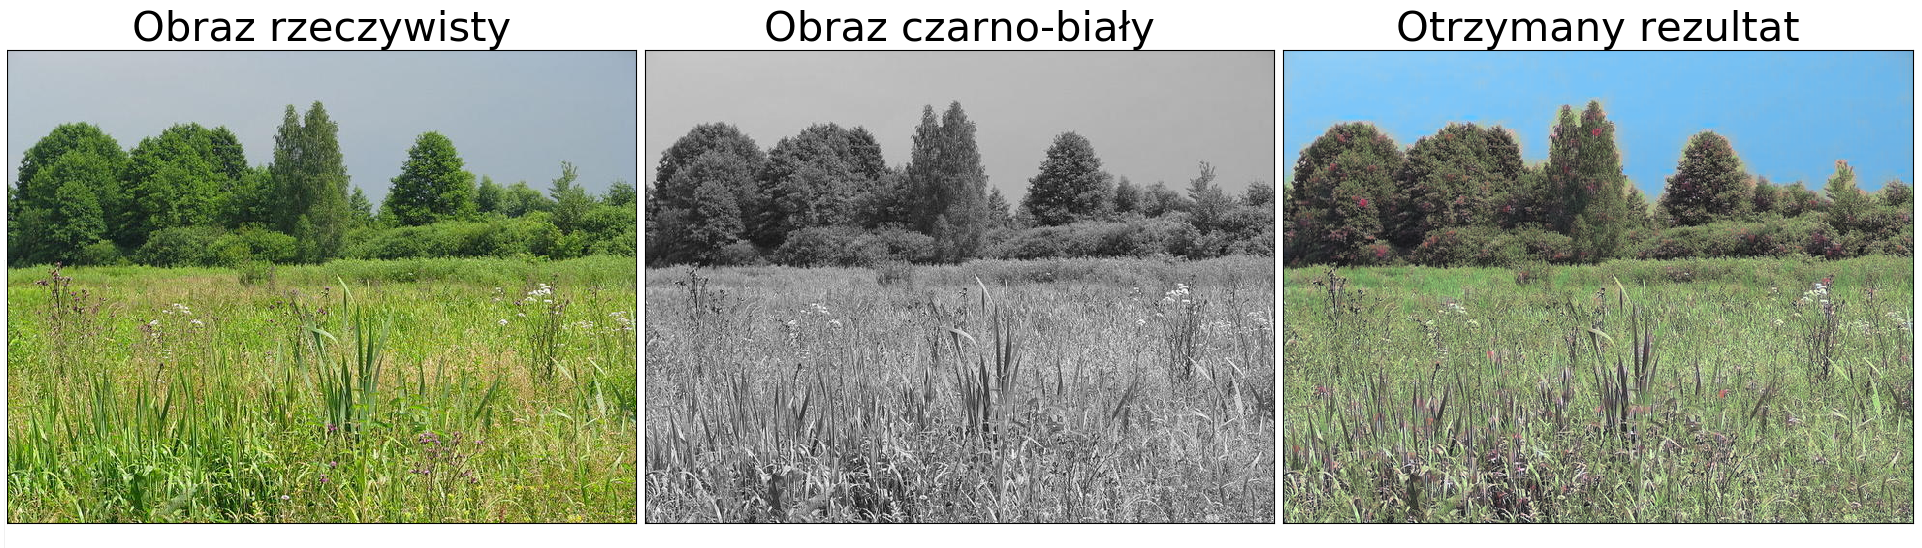
\includegraphics[width = 4.5in]{best_results_krajobraz}} \\
   \subfloat[Obraz ze zbioru uczącego]{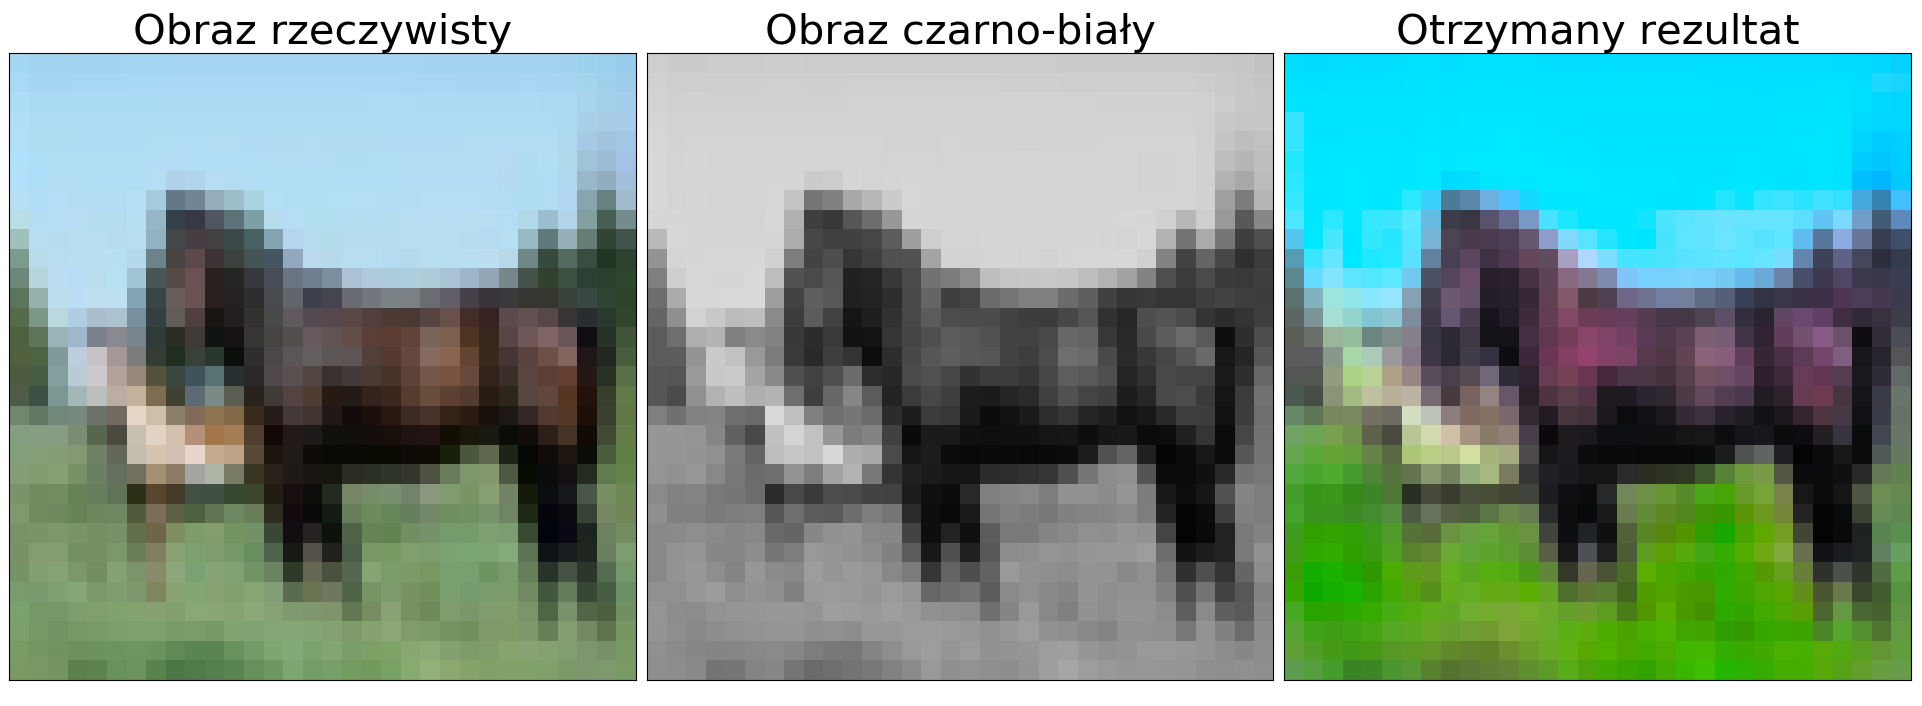
\includegraphics[width = 4.5in]{best_results_horse}} \\
   \caption[Efekty działania sieci - źródło: Rysunek własny bazujący na:
   \url{https://fr.m.wikipedia.org/wiki/Fichier:An_F-A-18C_Hornet_launches_from_the_flight_deck_of_the_conventionally_powered_aircraft_carrier.jpg},
   \url{https://pl.wikipedia.org/wiki/Plik:PL_Bagno_Calowanie_2.jpg}, \cite{cifar-10}]
   {Rezultaty.}
   \label{fig:best_result}
 \end{figure}

 \noindent
 Efekt ten został uzyskany przy następującej konfiguracji:
 \begin{itemize}
   \item Funkcja kosztu MSELoss.
   \item Funkcja aktywacji ReLU.
   \item Algorytm optymalizacyjny Adam.
   \item Normalizacja składowej \textit{L} podczas przetwarzania wstępnego.
   \item Standaryzacja składowych \textit{A} i \textit{B} podczas przetwarzania wstępnego.
   \item Nie zastosowanie rozmycia Gaussowskiego.
   \item Zastosowanie warstwy BatchNorm oraz nie zastosowanie warstwy Dropout.
   \item Zastosowanie zaproponowanego przez nas algorytmu przetwarzania końcowego.
 \end{itemize}

 \noindent
 Na podstawie obrazów na Rysunku \ref{fig:best_result} oraz przeprowadzonych
 testów można wywnioskować, że model nauczył się najlepiej kolorować powierzchnie
 o zazwyczaj stałej barwie takie jak niebo albo trawa, widać, że ich barwy są
 wyjątkowo intensywne oraz jednoznacznie wskazują co to są za powierzchnie.
 Gorzej rzecz się ma z obiektami o zmiennych barwach takimi jak na przykład
 samochody, w związku z ich zmienną barwą na przestrzeni całego zbioru danych
 model, chcąc zminimalizować błąd liczony przez funkcję kosztu, uśredniał kolor
 tych obiektów co skutkuje ich przytłumionymi barwami przechodzącymi często
 w odcienie brązu. Z tego powodu pomniejsze detale na kolorowanych zdjęciach
 tracą swoje barwy, efekty tego zjawiska można zaobserwować analizując
 stateczniki odrzutowca ukazanego na obrazie \textit{(a)} Rysunku \ref{fig:best_result}.
 Wykres uczenia przedstawionego modelu został przedstawiony na Rysunku
 \ref{fig:loss_plot}. Można zaobserwować stopniowy spadek wartości funkcji
 kosztu, co oznacza poprawne zbieganie się modelu do właściwego rozwiązania.
 W końcowych fazach wykresu widać, że wartość kary zmienia się o bardzo
 małe wartości, co znaczy, że proces uczenia wpadł już w minimum będące
 jednym z dostępnych rozwiązań.

 \begin{figure}[h]
  \centering
  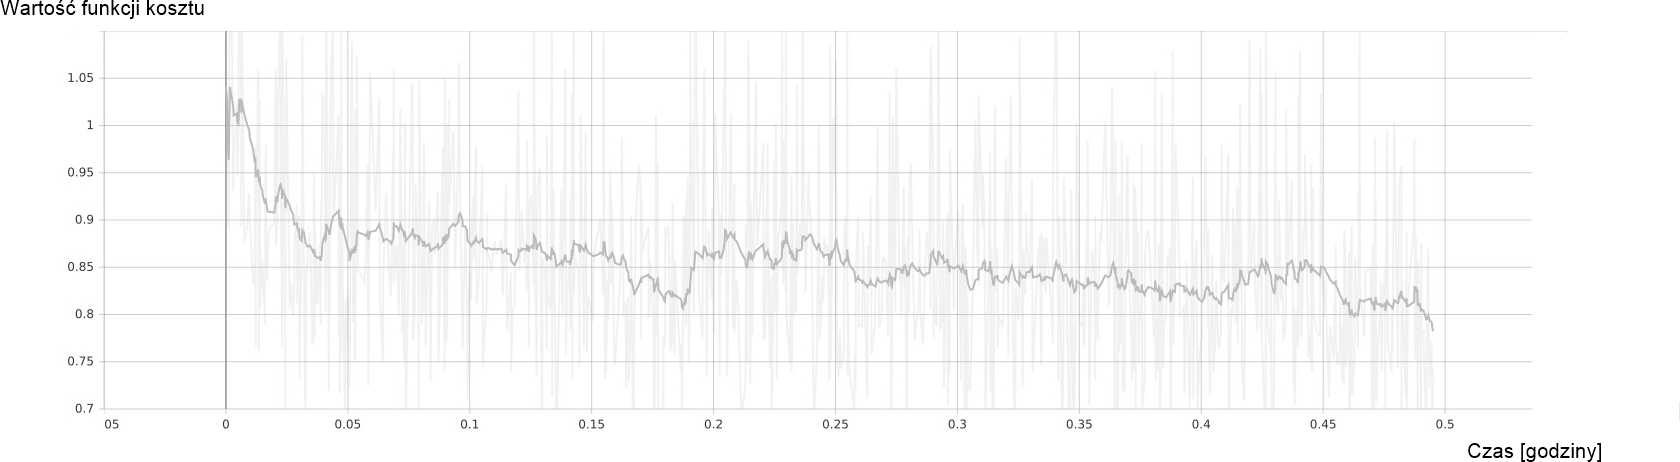
\includegraphics[width=6in]{loss_plot}
  \caption[Wykres uczenia modelu końcowego - źródło: Rysunek własny]
  {Wykres uczenia modelu końcowego}
  \label{fig:loss_plot}
 \end{figure}

  \noindent
  W dalszej części sekcji opisany został wpływ poszczególnych elementów konfiguracji.

  Największy wpływ na uzyskiwane rezultaty ma zastosowanie algorytmu przetwarzania
  końcowego opisanego w punkcie \ref{Przetwarzanie końcowe danych}. Pomógł on
  znacznie wzbogacić kolory generowane przez sieć. Odpowiednie porównanie
  zostało przedstawione na Rysunku \ref{fig:trick}. Wadami tej metody są generowane
  momentami zbyt intensywne barwy zdjęć oraz bardziej widoczne czasami
  zdarzające się "wycieki"
  kolorów jednych powierzchni na inne, przykładowo czerwony kolor z samochodu
  wychodzi poza powierzchnię samochodu i barwi fragmenty trawy przylegające do
  samochodu na czerwono. Efekt ten jest znacznie mniej widoczny przy zdjęciach
  o wysokiej rozdzielczości, co sprawia, że w zastosowaniu praktycznym ta
  wada modelu jest do zaakceptowania. Na Rysunku \ref{fig:trick} widać to
  poprzez drobne obszary żółci na granicy nieba i drzew.

  \begin{figure}[H]
   \centering
   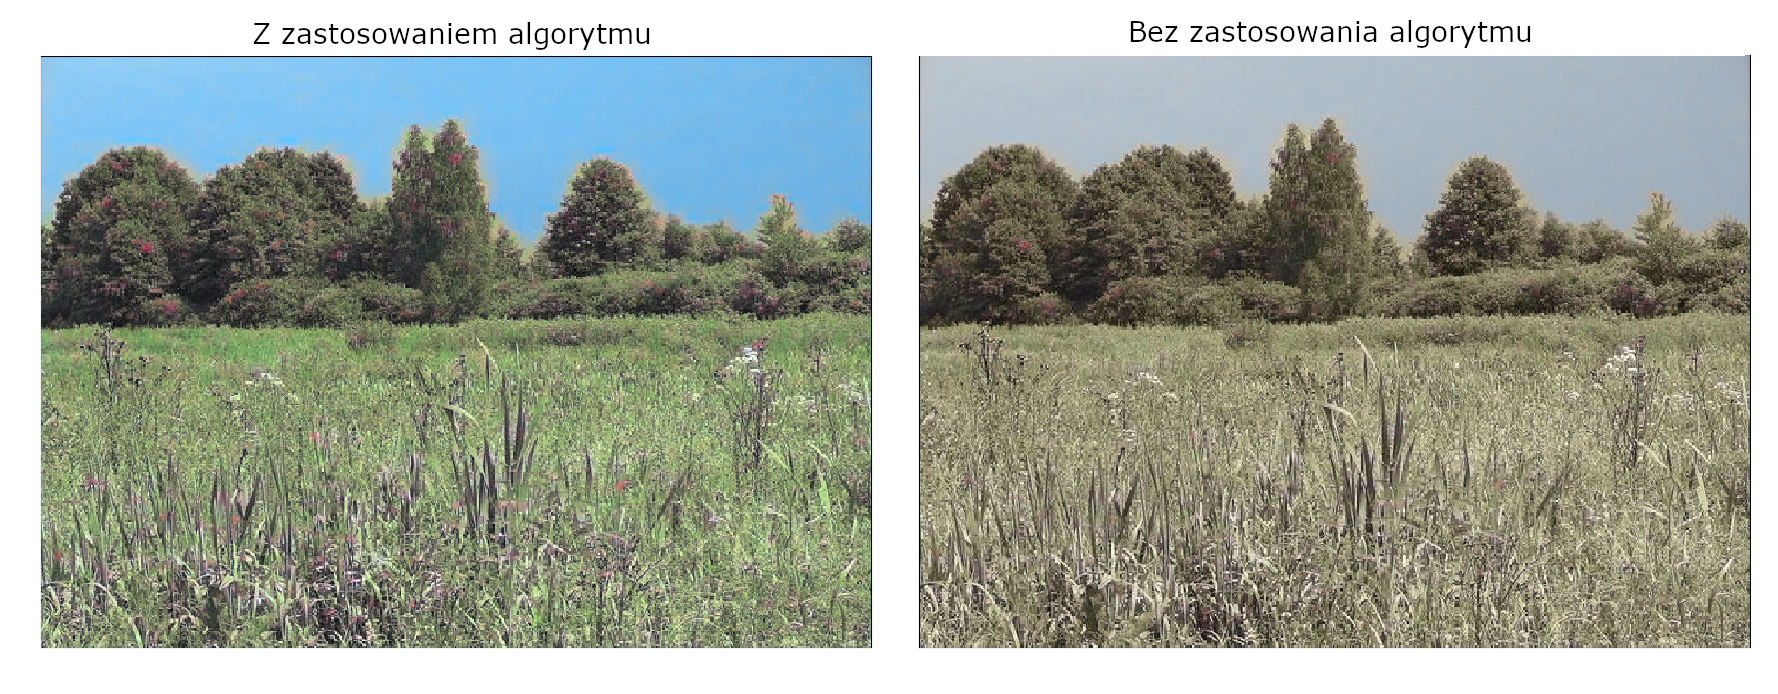
\includegraphics[width=6in]{porownania_trick_krajobraz}
   \caption[Efekt zastosowania algorytmu przetwarzania końcowego - źródło
   rysunek własny na podstawie: \url{https://pl.wikipedia.org/wiki/Plik:PL_Bagno_Calowanie_2.jpg}]
   {Efekt zastosowania algorytmu przetwarzania końcowego}
   \label{fig:trick}
  \end{figure}

  Kolejnym ważnym komponentem jest użyta funkcja kosztu, właściwy wybór
  znaczenie poprawia proces aktualizowania się wag sieci, co przekłada się
  na lepsze rezultaty. Kluczowe było, aby funkcja straty uwzględniała
  możliwą wielobarwność kolorowanych obiektów i nie karała sieci za barwy niezgodne
  z barwami na obrazie rzeczywistym, ale pasujące w kontekście kolorowanej
  powierzchni. Na Rysunku \ref{fig:porownanie_funkcji_kosztu} zostało
  umieszczone porównanie rezultatów modeli uczonych z użyciem różnych funkcji
  kosztu, przedstawione obrazy zostały wygenerowane bez użycia algorytmu
  końcowego przetwarzania w celu uwydatnienia cech funkcji kosztu.

  \begin{figure}[H]
   \centering
   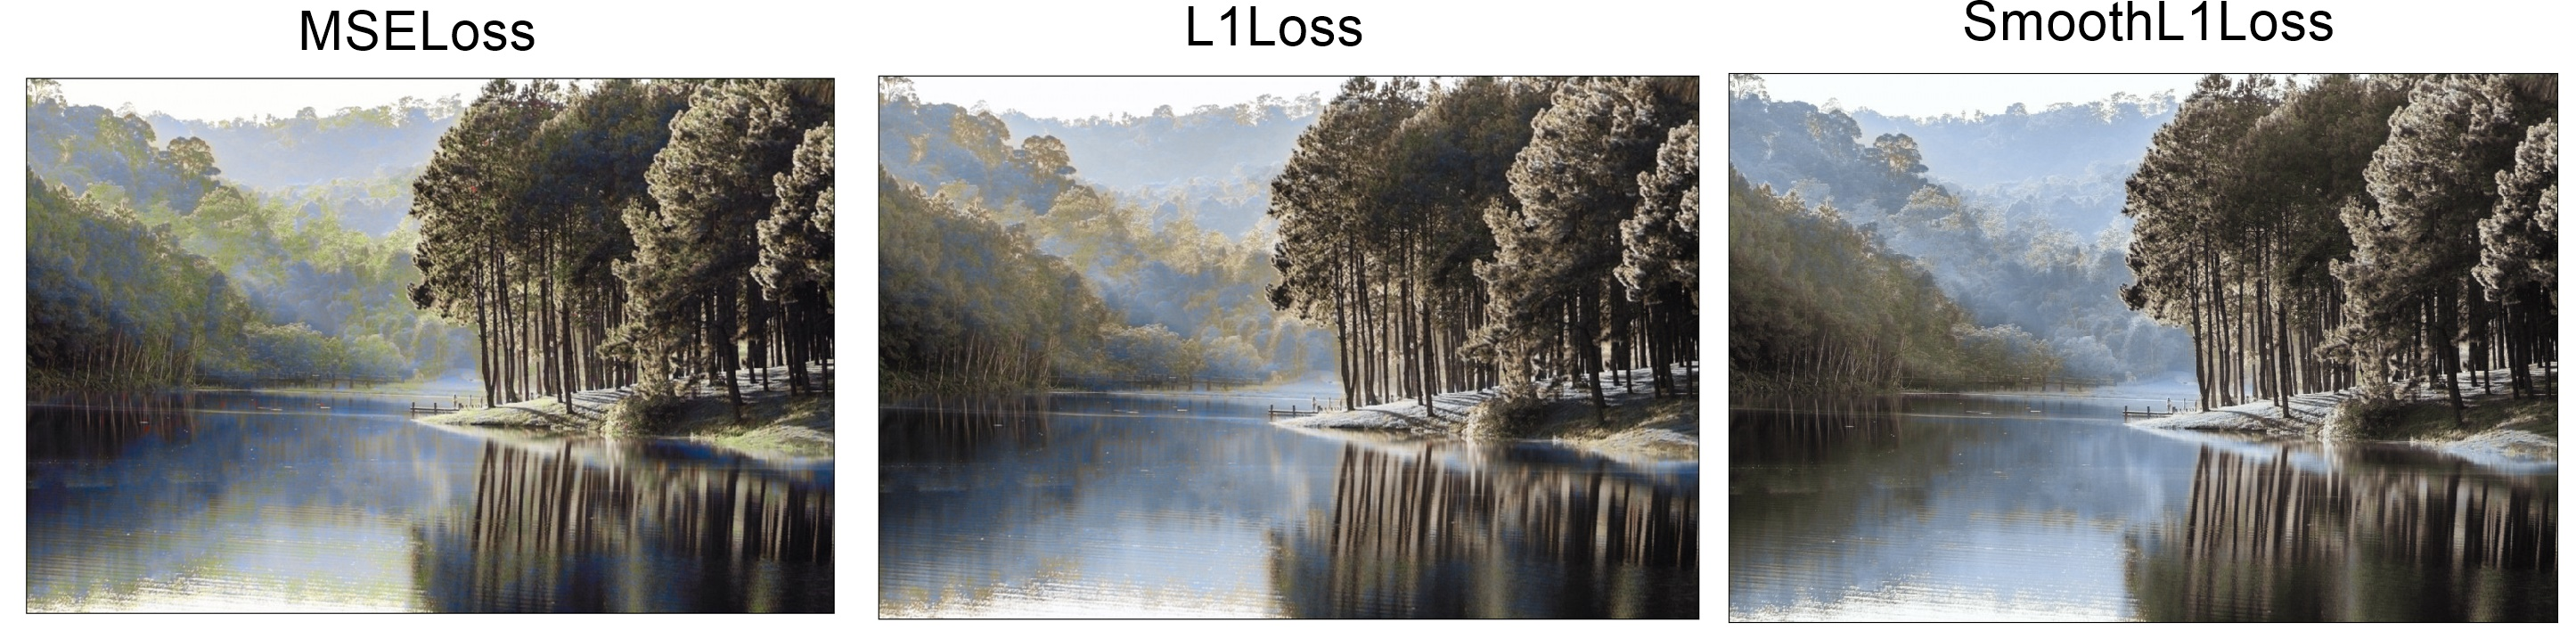
\includegraphics[width=6in]{porownanie_funkcji_kosztu}
   \caption[Porównanie rezultatów modeli uczonych z użyciem różnych funkcji
   kosztu - źródło rysunek własny na podstawie: \url{https://cdn.thearthunters.com/wp-content/uploads/2013/06/bg-960x636.jpg}]
   {Porównanie rezultatów modeli uczonych z użyciem różnych funkcji
   kosztu.}
   \label{fig:porownanie_funkcji_kosztu}
  \end{figure}

  \noindent
  L1Loss: Testując funkcję kosztu L1Loss oczekiwano, że uzyskiwane obrazy będą
  cechowały się niską saturacją, a generowane kolory będą przytłumione. Jest
  to spowodowane skłonnościami funkcji L1Loss do uśredniania wyjścia modelu w
  przypadku, kiedy kolorowana powierzchnia ma zmienną barwę na przestrzeni
  zbioru uczącego. Działanie L1Loss ma na celu zminimalizować błąd bezwzględny
  będący różnicą pomiędzy kolorami tych powierzchni, a kolorami generowanymi
  przez sieć, co skutkuje barwą o wartości znajdującej się pomiędzy wartościami
  wszystkich występujących kolorów dla powierzchni danego typu. W rezultacie
  otrzymywane są obrazy w kolorze sepii, co widać na Rysunku
  \ref{fig:porownanie_funkcji_kosztu}.

  \noindent
  SmoothL1Loss: Funkcja ta bazuje na L1Loss, ale tworzy kryterium, które przy
  błędzie bezwzględnym o wartości mniejszej niż 1 używa kwadratu z wartości
  błędu, a w pozostałych przypadkach używa wartości bezwzględnej błędu. Wzór
  L1Loss jest przedstawiony w punkcie \ref{Funkcje kosztów}. Zabieg ten sprawia,
  że funkcja jest mniej czuła na elementy odstające oraz przeciwdziała zjawisku
  eksplodującego gradientu. Funkcja to została zastosowana jako próba skuteczniejszego
  wyuczenia się przez model kolorów detali występujących na obrazach oraz aby przeciwdziałać
  uśrednianiu wartości barw przez sieć. Jednakże efekt ten nie został uzyskany,
  a przeciwdziałanie elementom odstającym przez SmoothL1Loss dodatkowo negatywnie wpłynęło na
  kolory generowane przez sieć. Funkcja wylicza mniejszy błąd, gdy
  wartość różnicy bezwzględnej pomiędzy wyjściem sieci, a kolorem
  rzeczywistym jest wysoka, co skutkuje tendencją modelu do
  generowania składowych \textit{A} i \textit{B} o wartościach ze środka
  przedziału wartości, czyli w okolicy zera. W praktyce jednak wartości tych
  składowych są ograniczane przez składową \textit{L} będącą jasnością obrazu,
  czego wynikiem są średnie wartości generowanych \textit{A} i \textit{B} lekko poniżej zera.
  Takie wartości odpowiadają głównie odcieniom niebieskiego i trochę odcieniom
  zielonego, co wyraźnie widać na Rysunku \ref{fig:porownanie_funkcji_kosztu}.

  \noindent
  MSELoss: W związku z brakiem algorytmu, który wstrzymuje karanie modelu w
  sytuacji, gdy generowane kolory są niezgodne z rzeczywistymi, ale prawdopodobne
  dla kolorowanej powierzchni to funkcja MSELoss również ma tendencję do
  uśredniania generowanych kolorów jak funkcja L1Loss. Jednakże większa czułość funkcji
  na wysokie wartości błędów, powodowana podnoszeniem różnicy pomiędzy wartością
  przewidzianą a rzeczywistą do kwadratu,
  umożliwiła wytrenowanie modelu zdolnego do generowania
  barw z szerokiego zakresu wartości, co korzystnie wpłynęło na rezultaty.
  Pokolorowany obraz wygenerowane przez model uczony z użyciem funkcji MSELoss prezentuje
  się najlepiej spośród obrazów na Rysunku \ref{fig:porownanie_funkcji_kosztu},
  z tego powodu oraz w związku z korzystnym efektem zastosowania MSELoss, właśnie
  ta funkcja została wybrana w procesie uczenia modelu końcowego.

  Wybór odpowiedniego algorytmu optymalizacyjnego może znacznie poprawić rezultaty
  modelu poprzez odpowiednie nakierowanie jego wag aby wartość kary wyliczana
  przez funkcję kosztu była jak najmniejsza. Minimalizowanie wartości tej kary
  jest zagadnieniem złożonym, w trakcie poszukiwania optimum dla wag sieci
  występują liczne minima lokalne, które utrudniają odnalezienie minimum '
  globalnego zapewniającego najbardziej satysfakcjonujące wyniki. Aby
  przeciwdziałać zatrzymaniu się procesu uczenia w lokalnych minimach należy
  zastosować odpowiedni algorytm optymalizacyjny. Przykładowy obraz pokolorowany
  przez model uczony z użyciem różnych algorytmów optymalizacyjnych został
  przedstawiony na Rysunku \ref{fig:porownanie_optimizerow}

  \noindent
  Dla algorytmu Adam zostały wybrane parametry: $\beta_{1} = 0.9$, $\beta_{2} = 0.999$,
  $\text{wskaźnik uczenia} = 0.1$, $\text{współczynnik zaniku wag} = 1e-10$ oraz
  $eps=1e-08$.
  \newline
  Dla algorytmu Adagrad zostały wybrane parametry: $\text{wskaźnik uczenia} = 0.1$,
  $\text{współczynnik zaniku wskaźnika uczenia} = 0.999$,
  $\text{współczynnik zaniku wag} = 1e-10$ oraz $eps=1e-10$.
  \newline
  Dla algorytmu SGD zostały wybrane parametry: $\text{wskaźnik uczenia} = 0.1$,
  $\text{pęd} = 0.9$, $\text{tłumienie} = 0$ oraz $\text{współczynnik zaniku wag} = 0$.
  Zmianę wskaźnika uczenia dla SGD nadzorował planista o parametrach:
  $\text{wielkość kroku} = 1$ oraz $\text{gamma} = 0.999$.

  \begin{figure}[H]
   \centering
   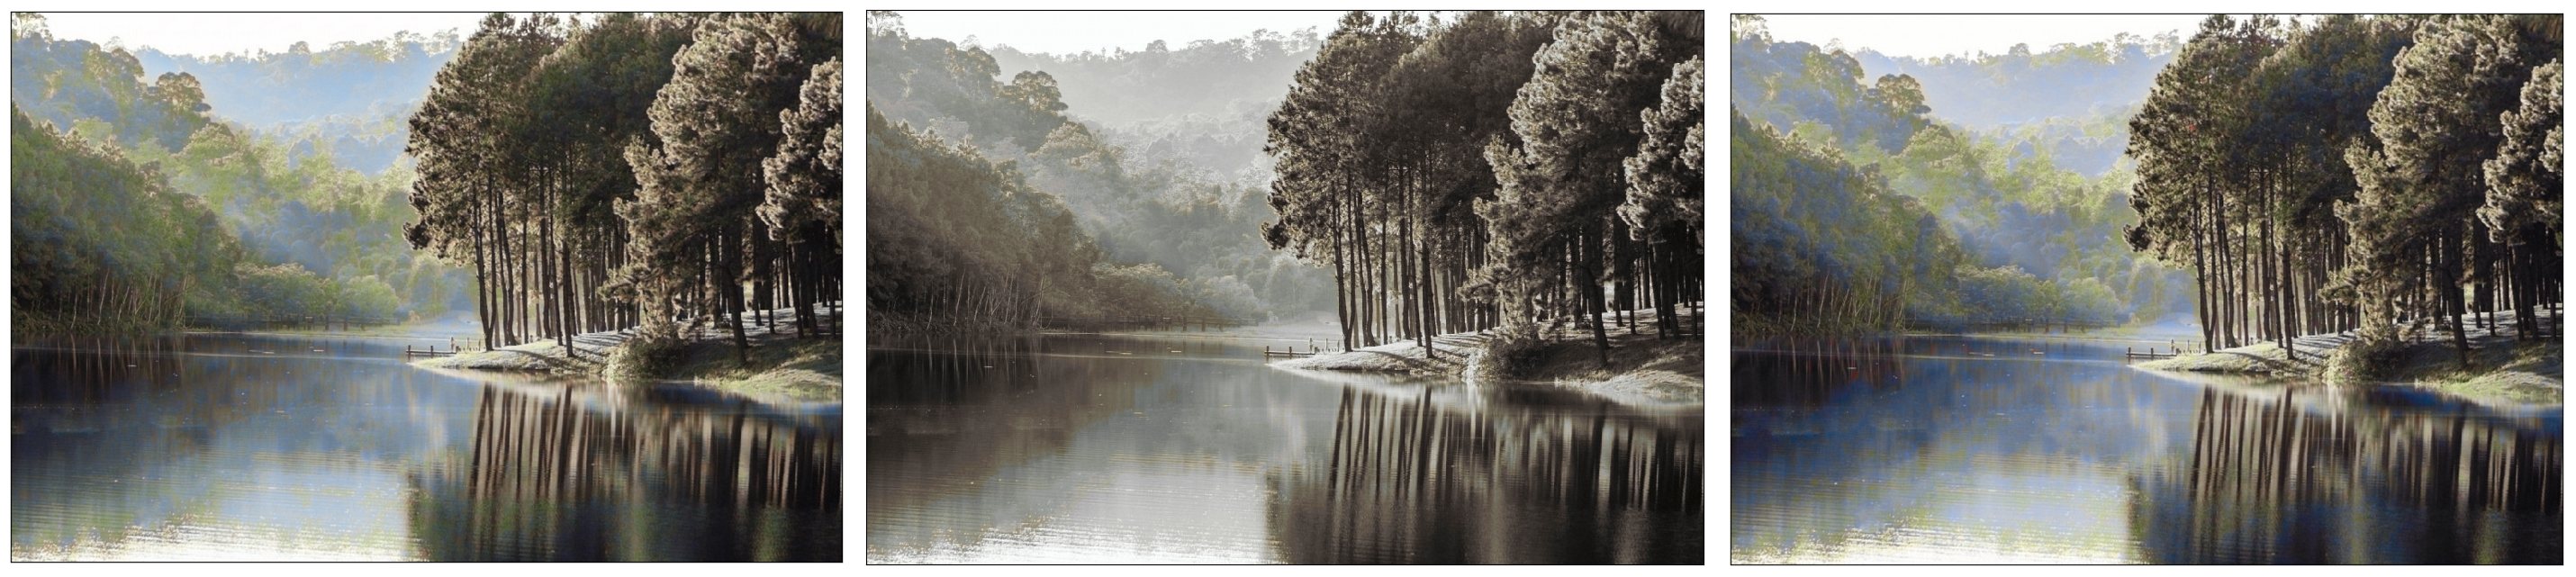
\includegraphics[width=6in]{porownanie_optimizerow}
   \caption[Porównanie rezultatów modeli uczonych z użyciem różnych algorytmów
   optymalizacyjnych - źródło rysunek własny na podstawie: \url{https://cdn.thearthunters.com/wp-content/uploads/2013/06/bg-960x636.jpg}]
   {Porównanie rezultatów modeli uczonych z użyciem różnych algorytmów
   optymalizacyjnych}
   \label{fig:porownanie_optimizerow}
  \end{figure}

  \noindent
  Jako algorytm optymalizacyjny dla modelu końcowego został wybrany Adam,
  decyzja ta jest oparta na wielu kryteriach takich jak wartości końcowe funkcji
  kosztu oraz wizualne efekty działania sieci. Przykładowa ocena wizualna
  została opisana bazując na Rysunku \ref{fig:porownanie_optimizerow}.
  Porównując pokolorowane obrazy można zauważyć, że najgorzej prezentuje się
  rezultat modelu stosujący algorytm Adagrad, na obrazie tym nie występuje wiele
  kolorów i dominują barwy szarości. Algorytm ten jest przeznaczony do
  pracy z rzadkimi zbiorami treningowymi, a zastosowany zbiór CIFAR-10 takim nie
  jest, można więc podejrzewać, że podczas procesu uczenia, wagi sieci na
  płaszczyźnie funkcji celu wpadły w minimum lokalne i nie były w stanie z niego
  wyjść, co poskutkowało pominięciem minimum globalnego będącego najlepszym
  możliwym rozwiązaniem. Analizując obrazy dla algorytmów Adam oraz SGD
  można zauważyć, że są one znacznie lepiej pokolorowane niż obraz dla
  algorytmu Adagrad. Można na nich wyraźnie wyróżnić roślinność pokolorowaną
  na zielono oraz taflę wody w odcieniach niebiskiego. Jednakże pomimo
  znacznego podobieństwa pomiędzy tymi dwoma obrazami można zauważyć, że tafla
  wody jest znacznie bardziej wypełniona kolorem na obrazie dla algorytmu Adam,
  co świadczy, że algorytm ten był w stanie zapewnić lepsze minimum dla wag
  sieci, co zapewniło modelowi lepiej rozwiniętą zdolność predykcji kolorów dla
  różnorodnych powierzchni.

  Z powodów opisanych w punkcie \ref{Dropout} warstwa Dropout nie została użyta
  w modelu autorskim. Na Rysunku \ref{fig:porownanie_dropout} został pokazany
  wpływ zastosowania tej warstwy w modelu na kolorowane przez model obrazy w zależności od
  wartości parametru \textit{p} (prawdopodobieństwo dezaktywowania dla każdego
  neuronu sieci).

  \noindent
  Jak widać zastosowanie tej warstwy nie przyniosło żadnych korzyści. Dla
  małych wartości parametru \textit{p} barwy na kolorowanym obrazie są
  mniej żywe niż bez zastosowania Dropout, a dla większych wartości widać, że
  model traci w dużej mierze swoje zdolności do predykcji kolorów. Dowodzi to,
  że w przypadku rozważanej problematyki większym zagrożeniem jest utrata
  kluczowych informacji o obrazie niż niebezpieczeństwo przeuczenia sieci, co
  sprawia, że warstwa Dropout staje się niepożądana.

  \begin{figure}[H]
   \centering
   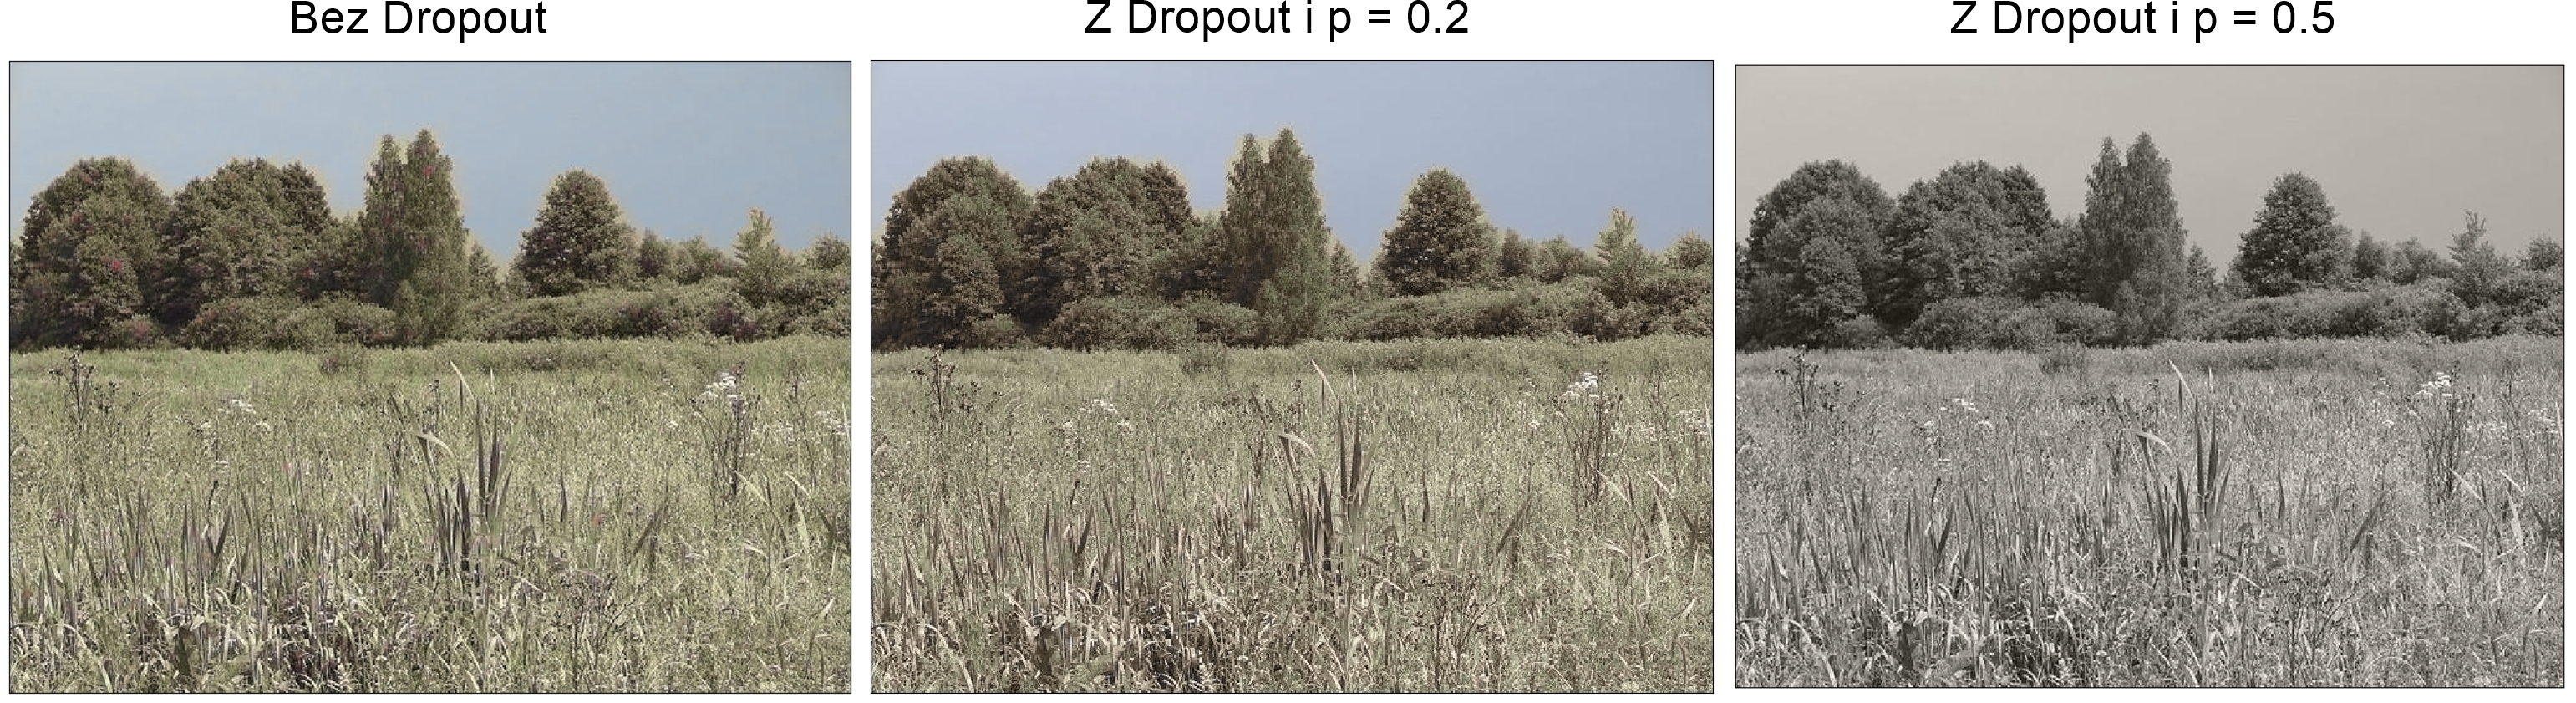
\includegraphics[width=6in]{porownanie_dropout}
   \caption[Wpływ zastosowania warstwy Dropout na kolorowanie obrazów - źródło: rysunek własny na podstawie:
   \url{https://pl.wikipedia.org/wiki/Plik:PL_Bagno_Calowanie_2.jpg}]
   {Wpływ zastosowania warstwy Dropout na kolorowanie obrazów}
   \label{fig:porownanie_dropout}
  \end{figure}

  Duże znaczenie dla jakości treningu modelu miał także wybór metod przetwarzania
  wstępnego zarówno obrazów wejściowych jak i obrazów referencyjnych. Przyczyny
  zastosowania takich zabiegów zostały dokładnie opisane w punkcie
  \ref{Przetwarzanie wstępne danych}.
  Porównanie efektów zastosowania różnych metod w różnych konfiguracjach zostało umieszczone
  na Rysunku \ref{fig:porownanie_preprocessing}, a dokładny opis konfiguracji
  został umieszczony w Tabeli \ref{table:preprocessing}.

  \begin{figure}[ht!]
    \centering
    \subfloat[]{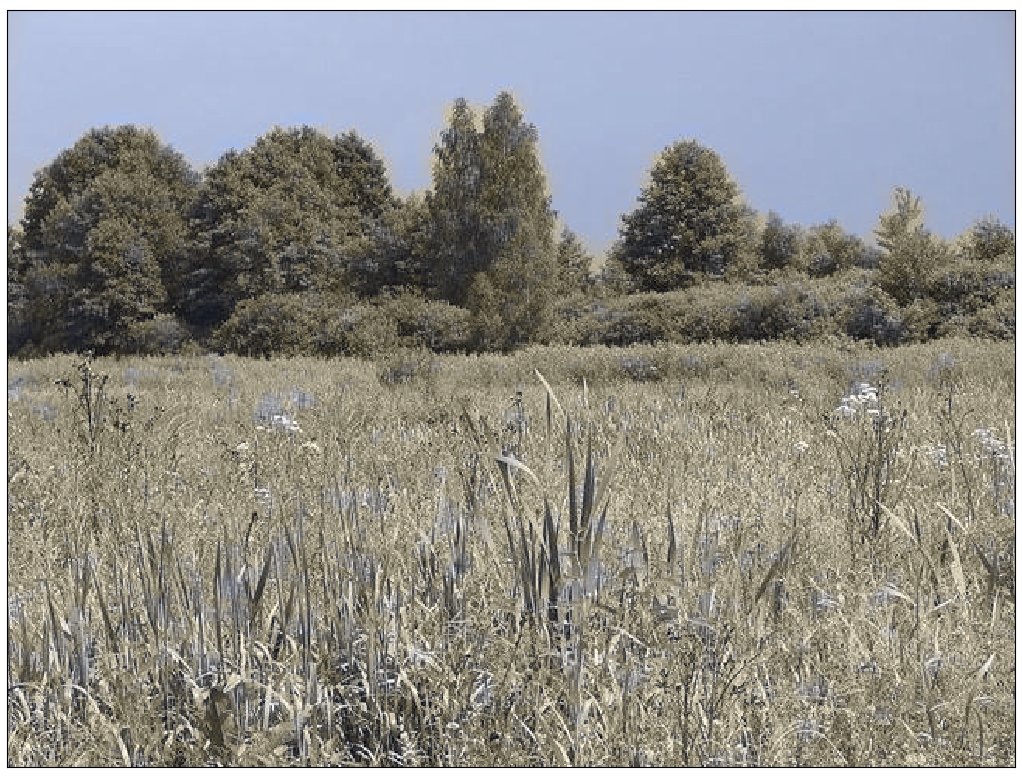
\includegraphics[width = 2in]{norm_norm}}
    \subfloat[]{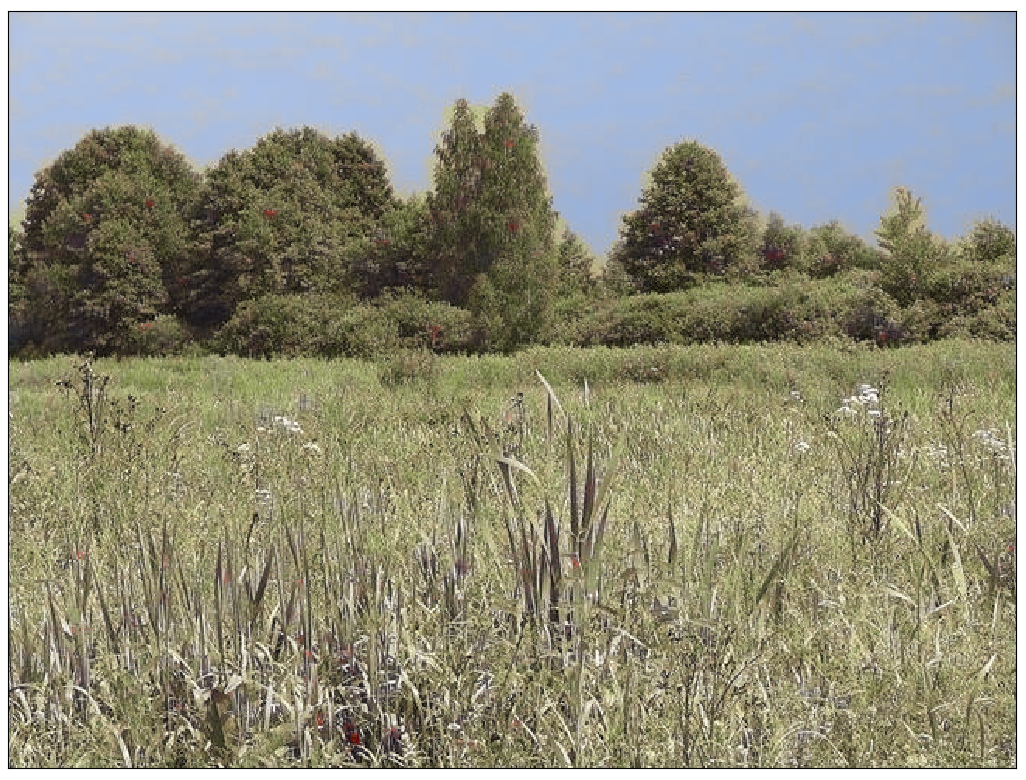
\includegraphics[width = 2in]{norm_stand}}
    \subfloat[]{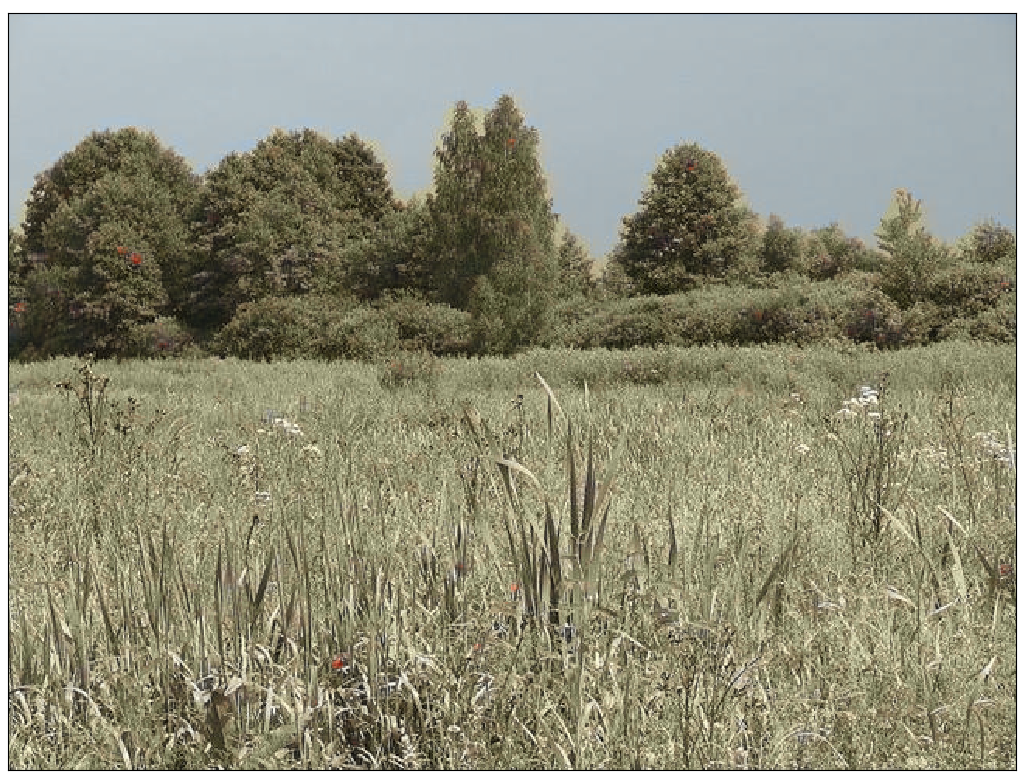
\includegraphics[width = 2in]{stand_stand}} \\
    \subfloat[]{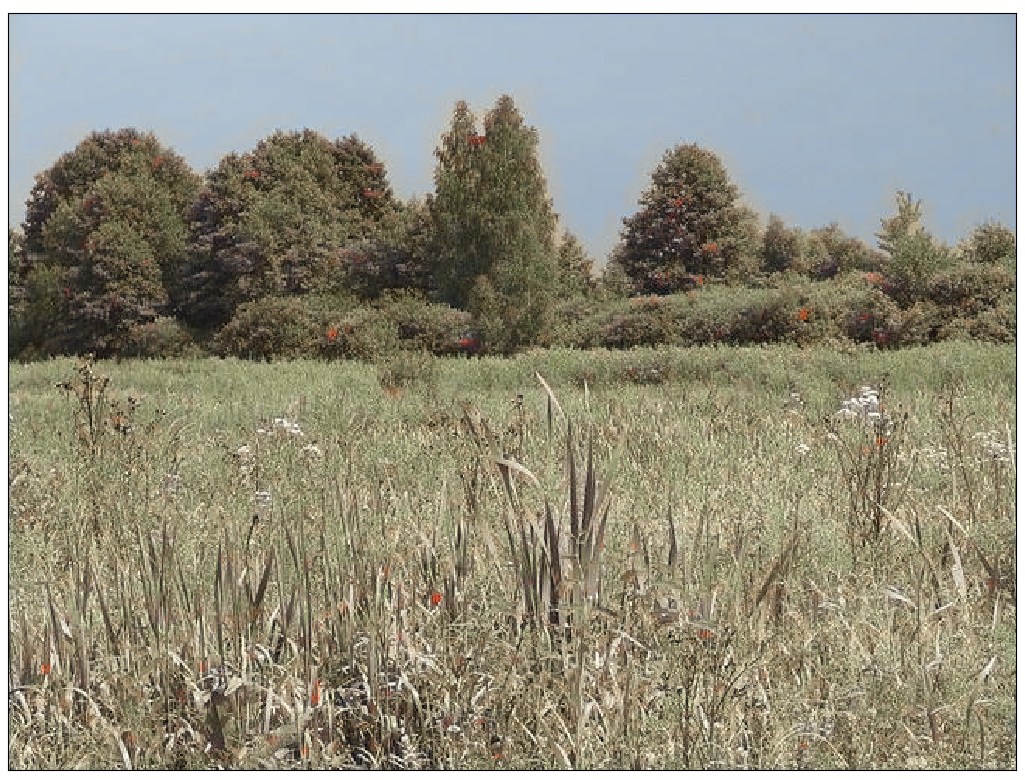
\includegraphics[width = 2in]{norm_stand_blur}}
    \subfloat[]{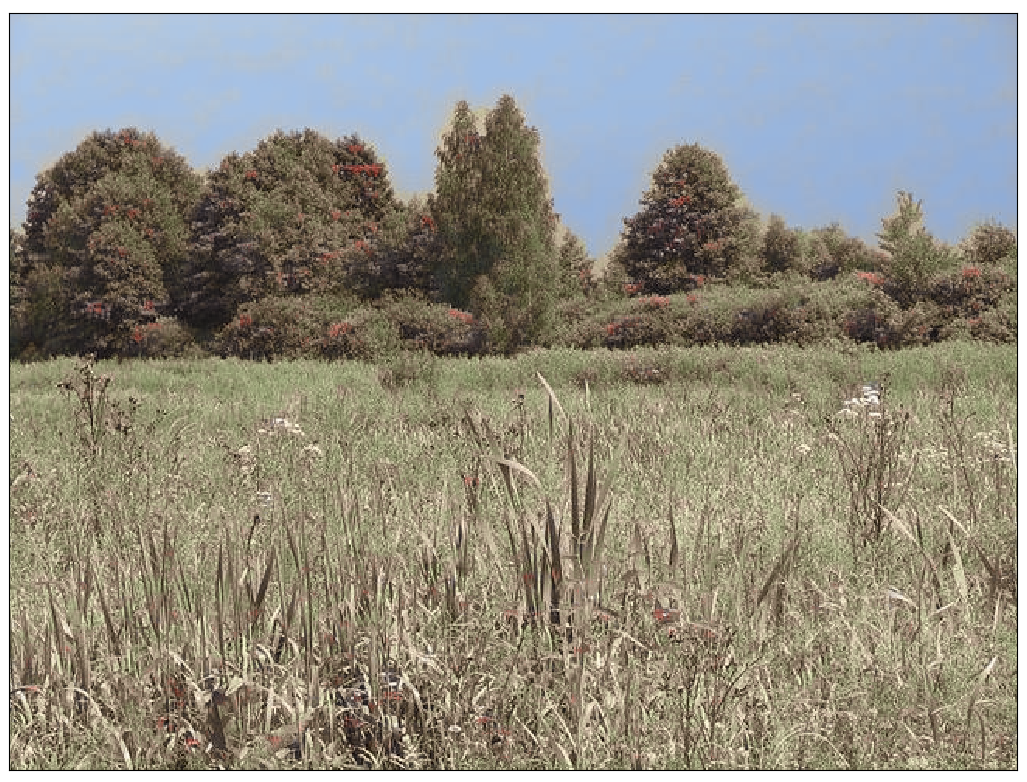
\includegraphics[width = 2in]{stand_stand_blur}} \\
    \caption[Skutki zastosowania różnych metod przetwarzania wstępnego - źródło:
    rysunek własny na podstawie
    \url{https://pl.wikipedia.org/wiki/Plik:PL_Bagno_Calowanie_2.jpg}]
    {Skutki zastosowania różnych metod przetwarzania wstępnego}
    \label{fig:porownanie_preprocessing}
  \end{figure}

  \noindent\begin{table}[H]
    \center
    \begin{tabular}{|c | c | c| }
     \hline
     Konfiguracja & Przetwarzanie danych wejściowych & Przetwarzanie danych
     referencyjnych \\ [0.5ex]
    \hline
    a & Normalizacja & Normalizacja \\ \hline
    b & Normalizacja & Standaryzacja \\ \hline
    c & Standaryzacja & Standaryzacja \\ \hline
    d & Normalizacja oraz rozmycie gaussowskie & Standaryzacja \\ \hline
    e & Standaryzacja oraz rozmycie gaussowskie & Standaryzacja \\ \hline
    \end{tabular}
    \caption{Szczegóły konfiguracji przetwarzania wstępnego.}
    \label{table:preprocessing}
  \end{table}

  \noindent
  Rezultaty przetwarzania wstępnego:
  \begin{enumerate}[label=(\alph*)]
    \item W pierwszej przetestowanej konfiguracji została zastosowana najprostsza
    metoda przetwarzania wstępnego - normalizacja, po jej zastosowaniu wartości wejścia sieci
    (składowa \textit{L}) oraz wartości referencyjne (rzeczywiste składowe
    \textit{A} i \textit{B}) były przeskalowane do przedziału od -0.5 do 0.5. Zabieg ten miał na
    celu usprawnić trening modelu z przyczyn opisanych w punkcie
    \ref{Przetwarzanie wstępne danych}. Jednakże można zauważyć, że rezultaty
    uzyskane przy tej konfiguracji prezentują się najgorzej w porównaniu z
    pozostałymi konfiguracjami, barwy na obrazie są przytłumione oraz mało
    różnorodne. Dowodzi to, że w przypadku rozważanej problematyki najprostsze
    rozwiązanie jest niewystarczające.
    \item W tym przypadku można zaobserwować znacznie lepsze rezultaty niż dla
    poprzedniej konfiguracji, Zastosowanie standaryzacji na danych referencyjnych
    znacznie usprawniło proces aktualizacji wag sieci w trakcie szukania minimum
    globalnego na płaszczyźnie funkcji celu. Generowane kolory są kontekstowo
    prawdopodobne dla kolorowanych powierzchni oraz cechują się wysokim stopniem
    nasycenia, co pozytywnie przekłada się na ich odbiór przez obserwatora. Ta
    konfiguracja została wybrana jako dająca najlepsze efekty z przedstawionych
    opcji.
    \item Kierując się sukcesem standaryzacji w konfiguracji (b) ocenione
    zostały rezultaty zastosowanie tej metody również dla danych wejściowych.
    Niestety zabieg ten nie przyniósł oczekiwanego polepszenia wyników
    modelu. Barwy na obrazie wyjściowym są mniej różnorodne oraz o
    niższej saturacji niż dla konfiguracji (b), ale za to o wyższej saturacji
    niż dla konfiguracji (a). Świadczy to, że w rozważanym zagadnieniu
    standaryzacja składowej luminacji nie wpływa pozytywnie na proces uczenia.
    Może to być spowodowane utratą kluczowych informacji o powiązaniach pomiędzy
    jasnością, a barwą, w przypadku przeskalowania składowej \textit{L}, tak aby
    uzyskać zerową wartość średnią oraz jednostkowe odchylenie standardowe.
    \item W tej konfiguracji została podjęta próba polepszenia rezultatów
    uzyskanych dla konfiguracji (b) poprzez zastosowanie dodatkowo rozmycia
    gaussowskiego na znormalizowanych danych wejściowych. Operacja ta miała na celu
    zmniejszyć wyraźność detali na obrazie, aby uwydatnić kluczowe cechy charakterystyczne
    powierzchni identyfikowanych przez warstwy konwolucyjne. Dzięki temu trenowany
    model miał się nauczyć rozpoznawać prawidłowo powierzchnie bez względu na
    przesłaniające je drobne obiekty oraz zawarte w tych powierzchniach detale
    nie zmieniające rodzaju tych powierzchni. Niepożądane by było,
    aby model inaczej nauczył się kolorować niebo w zależności czy na tle tego
    nieba występuje jakiś drobny obiekt taki jak ptak. Jednakże analizując
    Rysunek \ref{fig:porownanie_preprocessing} można dojść do wniosku, że nie
    przyniosło to oczekiwanych rezultatów, wbrew przeciwnie, obniżyło to jakość
    kolorowania względem konfiguracji bez rozmycia gaussowskiego, co wyraźnie
    widać po mniej intensywnych barwach na obrazie.
    \item Zastosowanie rozmycia gaussowskiego opisane dla konfiguracji (d)
    zostało także przetestowane w połączeniu z konfiguracją (c). W tym
    przypadku widać, że odniosło to pożądany efekt. Generowane kolory są znacznie
    bardziej nasycone niż dla konfiguracji (c) oraz pasują kontekstowo do
    powierzchni, na którą zostały nałożone. Wynika z tego, że w przypadku, kiedy zastosowanie
    standaryzacja na składowej \textit{L} może mieć niekorzystne skutki, to
    można je zredukować używają właśnie rozmycia gaussowskiego. Aczkolwiek
    porównując wyniki tej konfiguracji z wynikami konfiguracji (b) widać, że
    nie jest ona konfiguracją najbardziej odpowiednią dla rozważanego
    rozwiązania.
  \end{enumerate}

  \noindent
  Bazując na efektach wizualnych różnych konfiguracji do modelu końcowego
  została zastosowana konfiguracja (b) składająca się z operacji
  normalizacji składowej wejściowej sieci \textit{L} oraz standaryzacji
  referencyjnych składowych \textit{A} oraz \textit{B}.

  \subsubsection{Model autorski - wnioski}

  Analizując uzyskane rezultaty dla modelu końcowego, można stanowczo
  stwierdzić, że sieci FCN zdecydowanie nadają się jako rozwiązanie problematyki kolorowania
  czarno-białych obrazów. Ich niezwykłe zdolności do adaptacji oraz wyjątkowa
  biegłość w zapamiętywaniu i identyfikowanie istotnych wzorców świetnie współgrają
  przy generowaniu prawdopodobnych barw pasujących do kolorowanych powierzchni.
  Jednakże przedstawione rozwiązanie nie jest idealne, jego dużą wadą jest
  słabo rozwinięta umiejętność do kolorowania przez modeli drobnych detali na obrazach.
  Aby zniwelować tę wadę należałoby znacząco zmodyfikować model oraz podejście do
  danej problematyki.

  Jedno z potencjalnych modyfikacji mogłoby obejmować
  wprowadzenie segmentacji obrazu oraz klasyfikacji jego segmentów w celu
  zawężenia ilości potencjalnych barw prawdopodobnych dla analizowanego segmentu obrazu.
  Model w trakcie treningu uczyłby się możliwych kolorów oddzielnie dla wszystkich
  występujących na obrazach klas zamiast dla całego obrazu jako całość,
  zmniejszyłoby to wpływ obiektów na siebie nawzajem i prawdopodobnie zwiększyło
  zdolności sieci do kolorowanie pomniejszych detali występujących na obrazach.
  Ponadto umożliwiłoby to wykorzystanie większych oraz bardziej różnorodnych
  zbiorów treningowych, co zwiększyłoby uniwersalność tego rozwiązania.
  Jednakże takie podejście wymagałoby sieci o znacznie większej architekturze,
  co przekłada się na o wiele wyższe zapotrzebowanie na moc obliczeniową często
  ciężko dostępną bez wyspecjalizowanego sprzętu.

  Pomimo niedoskonałości przedstawionego modelu końcowego należy podkreślić jego
  użyteczność w półautomatycznym kolorowaniu czarno-białych obrazów. Jak można
  było zauważyć zadowalająco radzi sobie on z kolorowaniem tła obrazów oraz
  powierzchni o mało różnorodnej kolorystyce. Można wykorzystać to do wstępnego
  pokolorowania czarno-białego obrazu, a następnie tylko innymi metodami uzupełnić
  ubytki koloru oraz poprawić barwy wymagających tego detali. Takie podejście
  jest znacznie bardziej efektywne niż przykładowo kolorowanie obrazu ręcznie od
  początku do końca.


  \subsubsection{Model z wykorzystaniem przeniesienia uczenia}

  Olbrzymią zaletą sieci neuronowych, sprawiającą, że są one wyjątkowo
  uniwersalne, jest możliwość przenoszenia uczenia. Polega
  to na zastosowaniu w wybranym modelu wiedzy, którą inny model posiadł w trakcie
  treningu. Dzięki temu sieć trenowana do pewnego zadania z użyciem olbrzymich
  ilości danych może być wykorzystana w zadaniu podobnym, do którego nie
  posiada się zbyt wielu danych treningowych. Odbywa się to poprzez
  wyciągnięcie z wybranego modelu wyuczonych warstw specjalizujących się w
  pewnych operacjach oraz zastosowanie tych warstw w innym modelu, dzięki
  czemu można przykładowo uzyskać, bez konieczności treningu, warstwy konwolucyjne wytrenowane
  do wyciągania z obrazu jego kluczowych cech i identyfikowania charakterystycznych wzorców.
  Przenoszenie uczenia odbywa się poprzez zaimplementowanie w tworzonym modelu
  warstw na podobieństwo warstw modelu z użyciem którego chcemy dokonać
  przeniesienia uczenia, następnie dla tych warstw wczytuje się odpowiednie wagi
  z modelu już wytrenowanego.
  Takie działania dają olbrzymie możliwości konstruowania wyjątkowo złożonych i
  zaawansowanych modeli bez konieczności długiego ich treningu. Przenoszenie
  uczenia jest jedną z głównych metod znajdywania rozwiązań różnych problematyk
  z użyciem sieci neuronowych przy ograniczonych zasobach dostępnej mocy
  obliczeniowej oraz danych treningowych.

  Z związku z licznymi zaletami przenoszenia uczenia została podjęta próba
  zastosowania tej metody w
  zagadnieniu kolorowania czarno-białych obrazów. Do tego celu wykorzystane
  zostało podejście zaprezentowane przez L. Melas-Kyriazi oraz G. Han w 2016
  roku \cite{deconvolution_colorization}. Wykorzystali oni głęboką sieć
  splotową będącą połączeniem wyuczonej sieci typu ResNet
  (ang. Residual Networks) \cite{ResNet}
  z opracowanymi przez nich warstwami dekonwolucyjnymi. Model ten został
  zaimplementowany, a jego rezultaty zostały porównane z
  rezultatami modelu zaprezentowanego w punkcie \ref{model autorski}.

  Podobnie jak w modelu autorskim w procesie uczenia została wykorzystana przestrzeń
  barw CIELab. Na wejście sieci podawana była składowa jasności, a danymi
  referencyjnymi dla wyjścia sieci były dwie składowe koloru.
  Idea testowanej architektury
  polega na integracji cech wysokiego oraz średniego poziomu z przetwarzanego obrazu.
  Przykładowo cechy wysokiego poziomu mogą wskazywać na typ otoczenia, jeśli
  wykryte otoczenia okaże się pomieszczeniem to będzie to miało bezpośredni wpływ
  na cechy średniego poziomu, aby wskazywały, że w danej
  sytuacji niekorzystne jest kolorowanie powierzchni w barwach nieba albo trawy,
  a bardziej prawdopodobne będą barwy powiązane z wnętrzem pomieszczenia.
  Wykorzystany model składa się z 3 komponentów, sieci ResNet-Gray stanowiącej
  początkową część testowanego modelu, bloku fuzji oraz sieci dekonwolucyjnej
  odpowiedzialnej za wygenerowanie oczekiwanych kolorów.

  Model ResNet-Gray został opracowany przez autorów testowanego rozwiązania poprzez
  wytrenowanie modelu ResNet-18 do zadania klasyfikacji czarno-białych obrazów
  z użyciem zbioru danych ImageNet \cite{ImageNet}. Osiągnięta dokładność na zbiorze testowym
  była na poziomie 79.9\% w porównaniu z ResNet-18 klasyfikującym kolorowe obrazy z
  dokładnością 85\%. Pozwala to założyć, że model ResNet-Gray poprawnie nauczył
  się rozpoznawać najistotniejsze cechy obiektów na obrazach, co powinno
  przełożyć się na satysfakcjonującą jakość kolorowania.
  Zadanie ResNet-Gray w testowanym rozwiązaniu polega na identyfikacji
  na obrazie wejściowym kluczowych wzorców wymaganych do wyciągnięcia cech
  poszczególnych poziomów. Początkowe warstwy wyciągają cechy niskopoziomowe, takie jak położenie krawędzi na obrazie. Warstwy środkowe
  służą do odpowiedniego przetworzenia tych cech, aby uzyskać cechy średniopoziomowe,
  cechy te oprócz podania ich na kolejne warstwy ResNet-Gray są dodatkowo wyprowadzane
  na blok fuzji. Zadaniem ostatnich warstw jest wydobycie cech
  wysokiego poziomu, które również są przekazywane do bloku odpowiedzialnego za
  fuzję.

  Blok fuzji jest odpowiedzialny za przestrzenne połączenie podawanych
  na niego cech, a następnie przetworzenie ich przez sieć złożoną z jednej
  warstwy realizującej odpowiednią funkcję, której współczynniki poddawane są
  optymalizacji w procesie uczenia.

  Wyjście bloku fuzji jest następnie przekazywane na sieć dekonwolucyjną, która
  tworzy oczekiwane składowe \textit{A} i \textit{B} przestrzeni kolorów CIELab.
  Sieć ta składa się z zestawu członów konwolucyjnych i warstw nadpróbkujących
  (ang. upsampling). Ma ona na celu przetworzyć wejściowy zbiór cech otrzymany w
  procesie fuzji na składowe kolorów przewidzianych dla obrazu wejściowego.
  Każdy człon konwolucyjny, oprócz dwóch ostatnich, składa się z pojedynczej
  warstwy konwolucyjnej połączonej z warstwą BatchNorm i warstwą funkcji
  aktywacji ReLU. Przedostatni człon złożony jest z warstwy konwolucyjnej, po
  której umieszczona jest warstwa funkcji aktywacji Sigmoid, mająca na celu
  wygenerowanie oczekiwanych wartości dla składowych kolorów. Ostatni człon
  konwolucyjny składa się z pojedynczej warstwy konwolucyjnej, której wyjście
  przekazywane jest na ostatnią warstwę nadpróbkującą będącą zarazem wyjściem
  sieci dekonwolucyjnej.
  Warstwy nadpróbkujące w sieci służy do modyfikacji rozdzielczości kanałów
  przechodzących przez sieć, w tym rozwiązaniu zwiększają one
  dwukrotnie szerokość i wysokość każdego kanału wejściowego używając algorytmu
  najbliższego sąsiada.

  Wybrany loss i optimizer

  Wybrany preprocessing

  Rezultaty i porówniania
